\documentclass[dvipdfmx,runningheads]{llncs}
\setcounter{tocdepth}{3}
\usepackage{amssymb}
\usepackage{here}
\usepackage{enumitem}
\usepackage{algorithm}
\usepackage{algorithmic}
\usepackage{wrapfig}
\usepackage{tikz}
\usepackage{amsmath}
\usepackage{docmute}
\usetikzlibrary{automata}
\usetikzlibrary{arrows}
\usetikzlibrary{positioning}
\usetikzlibrary{lindenmayersystems}

\usetikzlibrary{decorations.markings}
\DeclareMathOperator*{\argmin}{arg\,min}
\title{Towards the Algorithmic Molecular Self-Assembly of Fractals by Cotranscriptional Folding\thanks{This work is in part supported by JST Program to Disseminate Tenure Tracking System, MEXT, Japan, No.~6F36 and by JSPS KAKENHI Grant-in-Aid for Young Scientists (A) No.~16H05854 to S.~S.}}
\titlerunning{Algorithmic Self-Assembly of Fractals by Cotranscriptional Folding}
\author{Yusei Masuda, Shinnosuke Seki, and Yuki Ubukata}
\institute{
Department of Computer and Network Engineering, 
The University of Electro-Communications, 
1-5-1, Chofugaoka, Chofu, Tokyo, 1828585, Japan \email{s.seki@uec.ac.jp}
}

\begin{document}

\maketitle

\begin{abstract}
RNA cotranscriptional folding has been recently proven capable of self-assembling a rectangular tile \textit{in vitro} (RNA origami). 
The oritatami system is a novel computational model of cotranscriptional folding. 
In this paper, we initiate the theoretical study on the algorithmic self-assembly of shapes by cotranscriptional folding using the oritatami system. 
We propose an oritatami system that folds into an arbitrary finite portion of the Heighway dragon, which is a fractal also-known as the paperfolding sequence $P = RRLRRLLR \cdots$. 
The $i$-th element of $P$ can be obtained by feeding $i$ in binary to a 4-state deterministic finite automaton with output (DFAO). 
We implement this DFAO and a bit-sequence bifurcation component as modules of oritatami system. 
Combining them with a known binary counter module yields the proposed oritatami system. 
\end{abstract}


%-------------------------------------------------------------------------------------------
	\section{Introduction}
%-------------------------------------------------------------------------------------------

An RNA sequence, over nucleotides of four kinds {\tt A}, {\tt C}, {\tt G}, {\tt U}, is synthesized (\textit{transcribed}) from its template DNA sequence over {\tt A}, {\tt C}, {\tt G}, {\tt T} nucleotide by nucleotide by an RNA polymerase (RNAP) enzyme according to the one-to-one mapping ${\tt A} \to {\tt U}$, ${\tt C} \to {\tt G}$, ${\tt G} \to {\tt C}$, and ${\tt T} \to {\tt A}$ (for details, see, e.g., \cite{AJLMRRW2014}). 
The yield, called \textit{transcript}, starts folding immediately after it emerges from RNAP. 
This is the \textit{cotranscriptional folding} (see Fig.~\ref{fig:rna_origami}). 
Geary, Rothemund, and Andersen have recently demonstrated the capability of cotranscriptional folding to self-assemble an RNA molecule of an intended shape at nano-scale \cite{GearyRothemundAndersen2014}. 
They actually proposed an architecture of a DNA sequence whose transcript folds cotranscriptionally into an RNA tile of specific rectangular shape highly likely \textit{in vitro}. 

\begin{figure}[tb]
\centering
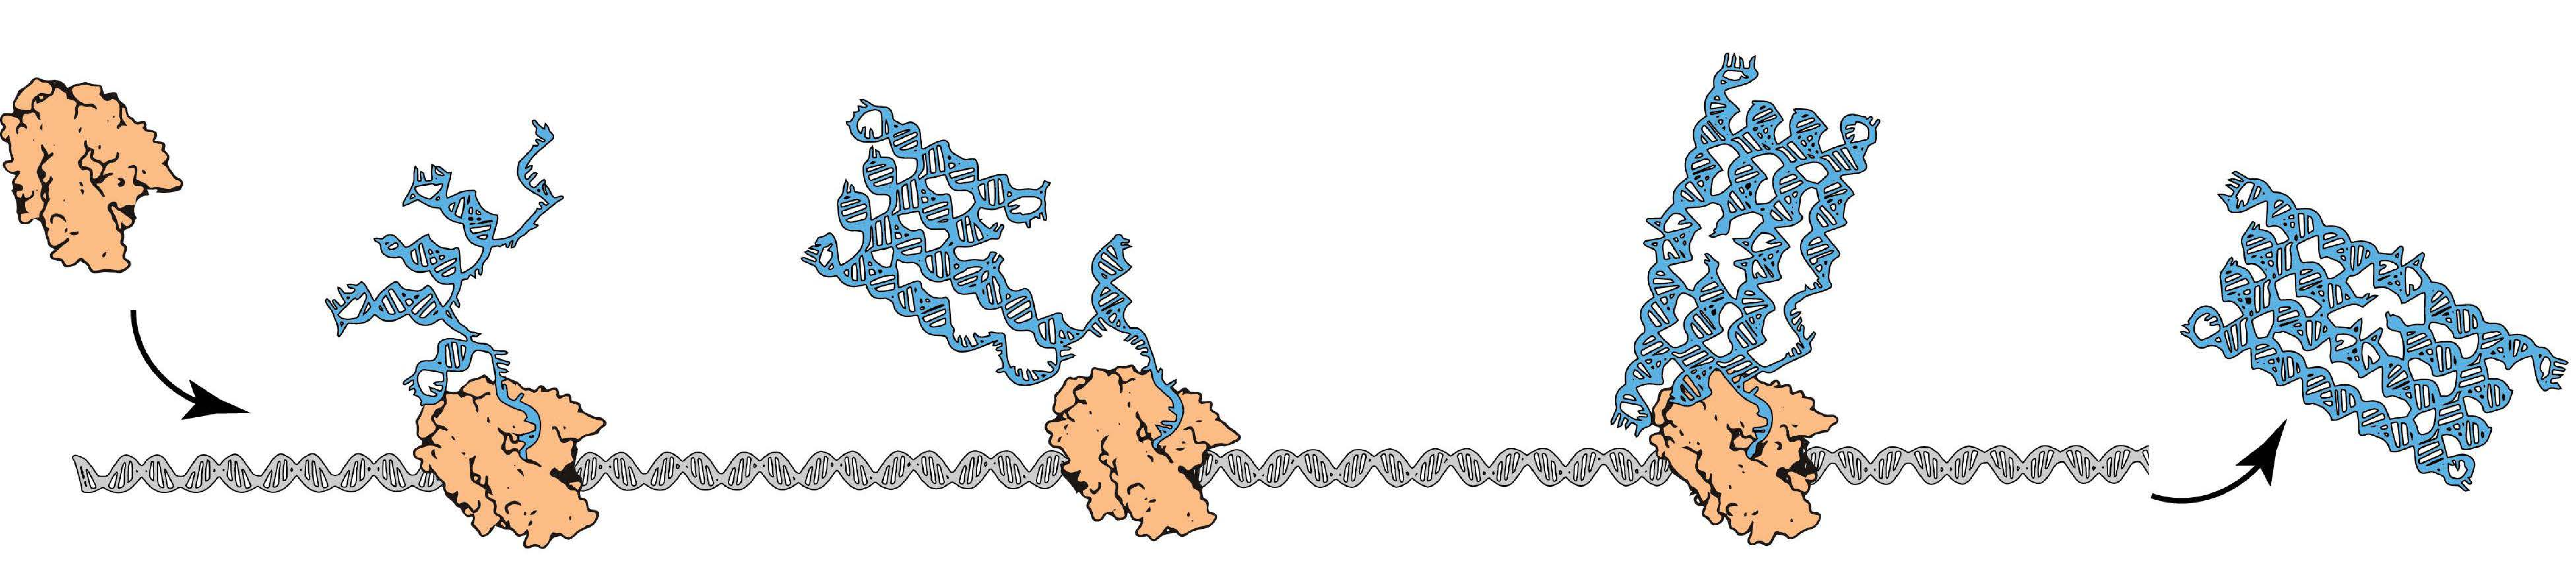
\includegraphics[width=0.8\linewidth]{pic/rna_origami.pdf}
\caption{RNA cotranscriptional folding. 
An RNA polymerase attaches to a template DNA sequence (gray spiral), scans it through, and synthesizes its RNA copy. 
The RNA sequence begins to fold upon itself immediately as it emerges from polymerase. 
}
\label{fig:rna_origami}
\end{figure}

%In this paper, we shall initiate the theoretical study on algorithmic self-assembly of shapes by cotranscriptional folding using a novel computational model of cotranscriptional folding called the \textit{oritatami system} \cite{GeMeScSe2016}.
Algorithms and computation are fundamental to molecular self-assembly as illustrated in an enormous success of their use in DNA tile self-assembly (see, e.g., \cite{Doty2012,Patitz2016,WinfreePhD} and references therein). 
%The concepts of computation and algorithms are yet to be as much utilized in the self-assembly of shapes by cotranscriptional folding as in the DNA tile self-assembly, where for example 
The Sierpinski triangle fractal was algorithmically self-assembled even \textit{in vitro} from coalescence of DNA tiles that compute XOR \cite{RothemundPapadakisWinfree2004}. 
Cotranscriptional folding exhibits highly sophisticated computational and algorithmic behaviors as well. 
Indeed, fluoride riboswitches in \textit{Bacillus cereus} bacteria cotranscriptionally fold into a terminator stem or does not in order to regulate gene expression \cite{WaStYuLiLu2016}. %depending on ligand concentration \cite{WaStYuLiLu2016}. 
This is just one example but should be enough to signify the context-sensitivity of cotranscriptional folding and shapes thus self-assembled. 
Geary et al.~have proved the capability of context-sensitivity to count in binary using a novel mathematical model of cotranscriptional folding called \textit{oritatami system} (abbreviated as OS) \cite{GeMeScSe2016}. 

%Cotranscriptional folding is in fact proved Turing-universal by the oritatami system \cite{GeMeScSe2015}. 
%The Turing-machine simulator is gigantic and intricate but oritatami systems have implemented basic computational devices such as binary counter \cite{GeMeScSe2016} as a module comparable in size to the gene expression regulator. 
%The binary counter module consists of half-adder components, which fold into one of possible four conformations depending on a 1-bit input and a 1-bit carry/non-carry encoded in their surroundings somehow. 
%It can be diverted as a copier for binary sequences by being fed with the non-carry. 
%They shall be reused in this paper. 

\begin{figure}[tb]
\centering
\begin{minipage}{0.4\linewidth}
\centering
\scalebox{0.7}{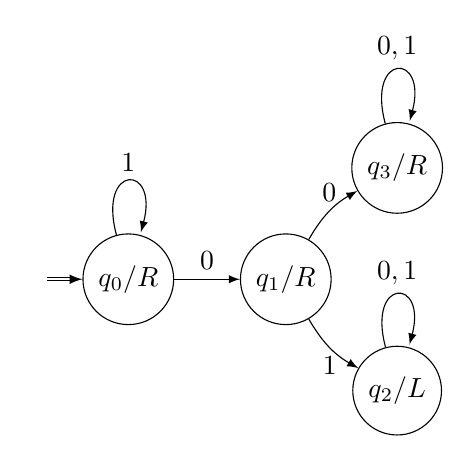
\begin{tikzpicture}[>=latex, node distance=2cm, initial text=, bend angle=15]
	\tikzstyle{every initial by arrow} = [->, double];

	\node [state, initial] (q_0)                        {$q_0/R$};
	\node [state]                     (q_1) [right of = q_0]  {$q_1/R$};
	\node [state]                     (q_2) [below right of = q_1] {$q_2/L$};
	\node [state]                     (q_3) [above right of = q_1] {$q_3/R$};

	\path [->] (q_0) edge [right] node [above]              {$0$}                 (q_1)
         		         edge [loop above] node [above]             {$1$}               ()
         			   (q_1) edge [bend left] node [above]             {$0$}                 (q_3)
         		         edge [bend right] node [below]             {$1$}              (q_2)
         			   (q_2)  edge [loop above] node [above]             {$0,1$}               ()
         			   (q_3)  edge [loop above] node [above]             {$0,1$}               ();
\end{tikzpicture}}
\end{minipage}
\begin{minipage}{0.05\linewidth}
\ \\
\end{minipage}
\begin{minipage}{0.5\linewidth}
\centering
\scalebox{0.03}{
\begin{tikzpicture}
  \draw[blue!50!black,rotate=270,l-system={rule set={X->X-YF,Y->FX+Y},
  step=100pt,angle=90,axiom=FX,order=10},-triangle 90] l-system;
\end{tikzpicture}}
\end{minipage}
\caption{
%Heighway dragon. 
(Left) DFAO to output the direction (L/R) of $i$-th turn of the Heighway dragon given $i \ge 0$ in binary from the LSB. 
(Right) The first $2^{10}{-}1$ turns of the dragon. 
}
\label{fig:heighway_dragon}
\end{figure}

We shall initiate theoretical study on algorithmic self-assembly of shapes by cotranscriptional folding using oritatami system. 
Sierpinski triangle would allow our study to borrow rich insights from the DNA tile self-assembly. 
However, in order to cut directly to the heart of algorithmic self-assembly by cotranscriptional folding, shapes of choice should be traversable somehow algorithmically. 
One such way is to feed a turtle program (see \cite{AbelsondiSessa1981}) with an \textit{automatic sequence} as commands (drawing a line segment, rotation, etc.), whose $i$-th bit can be obtained by giving $i$ in binary from the least significant bit (LSB) to one DFA with output (DFAO) \cite{AlloucheShallit2003}.
Shapes thus describable include the Heighway dragon \cite{AlloucheShallit2003} and von Koch curve \cite{MaHoldener2005}. 
A DFAO for the Heighway dragon (Fig.~\ref{fig:heighway_dragon}) outputs the following sequence, given $i = 0, 1, 2, \ldots$ in binary: 
%It is to read the binary representation of $i \ge 0$ from the LSB and outputs the $i$-th direction $P[i]$ to turn (L or R) assigned to the state finally reached as follows: 
\[
%\begin{array}{cccrrrrc}
%i 	&=& 0 &  2 & 6 & 14 & 30 & \cdots \\
%P[i] 	&=& {\rm R} & {\rm RL} & {\rm RRLL} & {\rm RRRLLRLL} & {\rm RRRLRRLLLRRLLRLL} & \cdots.
%\end{array}
P 	= {\rm RRLRRLLRRRLLRLLRRRLRRLLLRRLLRLL} \cdots.
\]
(The notation $P$ is after its appellative \textit{paperfolding sequence} \cite{AlloucheShallit2003}.) 
For instance, $i = 2$ is given in binary from the LSB as 01, with which the DFAO transitions as $q_0 \to q_1 \to q_2$ and hence $P[2] = L$. 
%where only the values of $i$ at the end of the first five iterations are specified. 
A turtle should interpret an L (resp.~R) as ``move forward by unit distance and turn left (resp. right) 90 degrees.''
Any portion of the dragon can be represented by a factor of $P$; for instance, Fig.~\ref{fig:heighway_dragon} (Right) depicts the factor $P[0 .. 1022]$, i.e., the first $2^{10}-1$ turns of the dragon. 

%\begin{figure}[htb]
\begin{wrapfigure}{l}{0.57\linewidth}
\vspace*{-5mm}
\centering
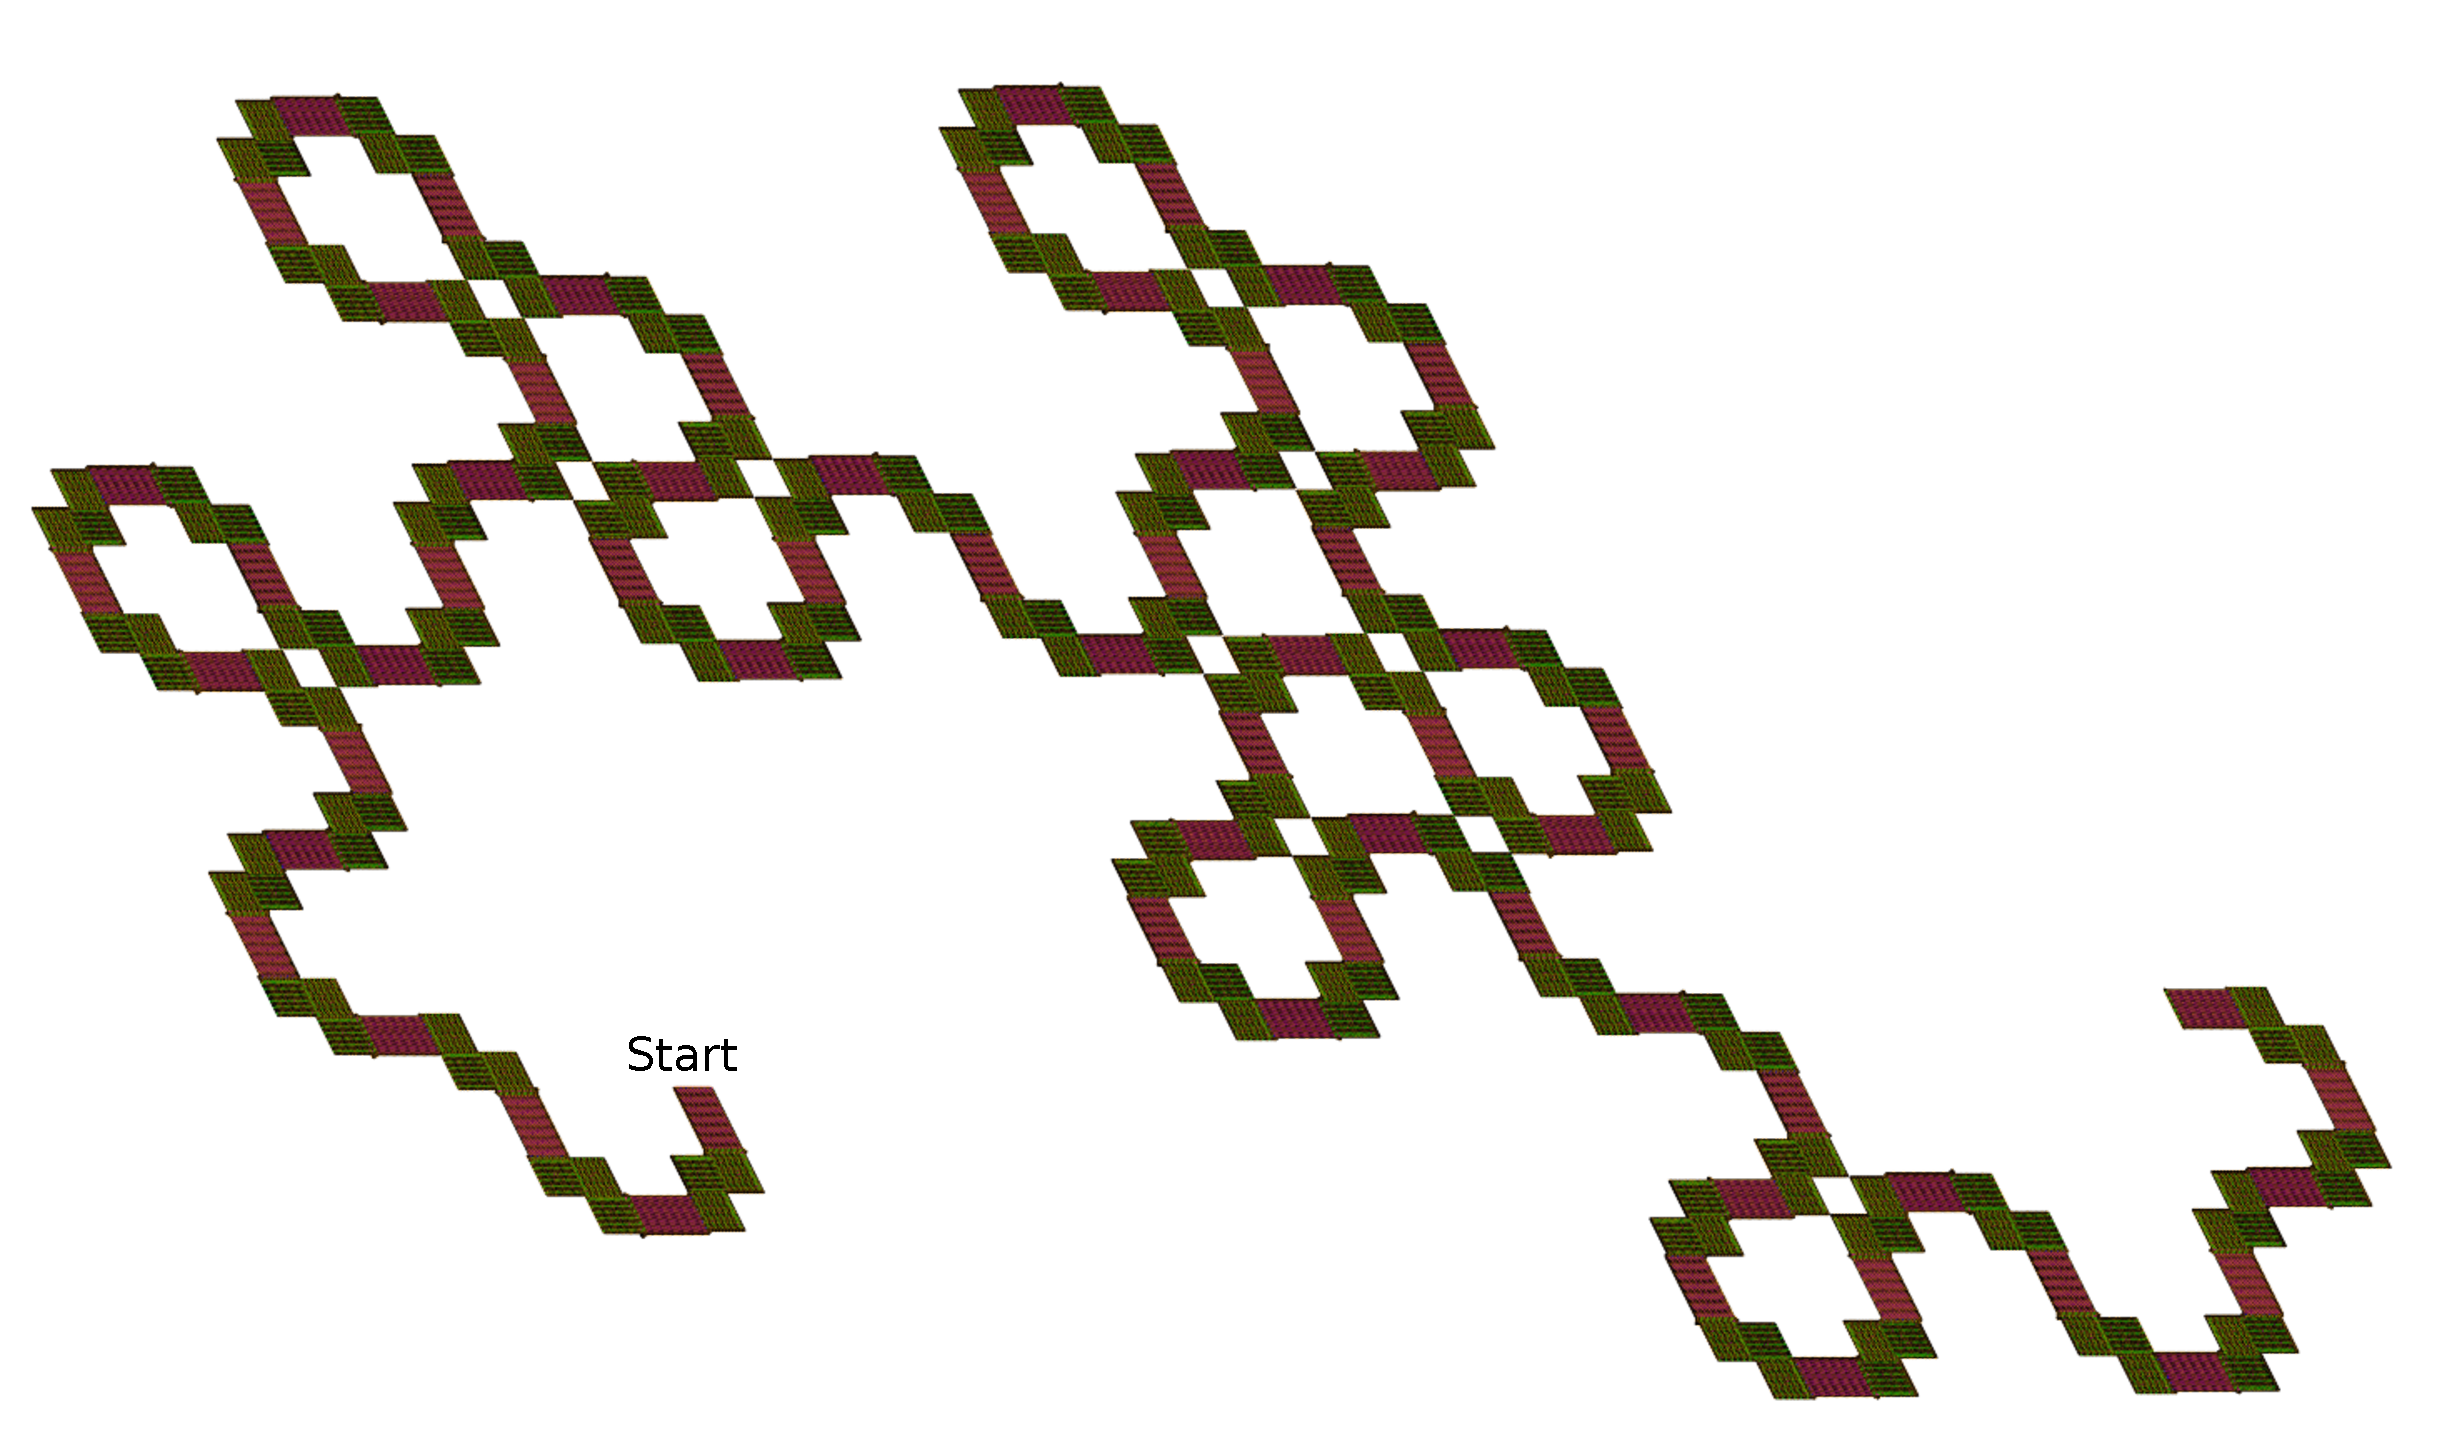
\includegraphics[width=\linewidth]{pic/6bit_heighway.pdf}
\caption{The portion $P[0 .. 62]$ of the Heighway dragon folded by the proposed oritatami system.}
\label{fig:heighway6_oritatami}
\vspace*{-5mm}
\end{wrapfigure}
%\end{figure}

In this paper, we propose a generic design of oritatami system for the algorithmic cotranscriptional folding of an arbitrary finite portion of the Heighway dragon. 
Fig.~\ref{fig:heighway6_oritatami} shows the portion $P[0 .. 62]$ thus folded (the dragon is slanted but this is because the OS operates on the triangular grid). 
The transcript is a repetition of three modules: a catenation of binary counters, DFAO module, and turning module. 
The counter is a technical modification of the one proposed in \cite{GeMeScSe2016}. 
By being fed with carry exactly once, the catenation increments the count $i$ exactly by 1 while folding into a (red) line segment. 
%It folds into one zigzag and increments a given binary number by 1 if carried-in or just propagates the number otherwise. 
%Binary counters fold into zigzags, yielding a (red) line segment of the dragon. 
%The system feeds only the first counter with carry so that the line segment amounts to increment the current count $i$ by 1. 
At the end of the segment comes a DFAO module, which computes the turn direction $P[i]$, reinterprets it properly as A/O, and propagates the count $i$ for the next turning module. 
A (green) L-shaped block is the turning module. 
It is a concatenation of three bit-sequence bifurcators, each of which folds into a rhombus, bifurcates $i$ leftward as well as rightward, and guides further folding according to A/O. 
%We shall implement the DFAO and turning modules and verify them. 

The generic design proves the next theorem (for terminologies, see Sect.~\ref{sect:preliminaries}). 

\begin{theorem}\label{thm:main}
	For any finite portion $P[i..j]$ of the Heighway dragon, there exist an integer $c$ and a deterministic cyclic oritatami system of delay 3 and arity 3 that weakly folds into the $c$-rhombus scaling of $P[i..j]$. 
\end{theorem}

\noindent
A JavaScript program to run this OS is available at {\small {\tt https://wolves13.github.io}}. 


%-------------------------------------------------------------------------------------------
	\section{Preliminaries}
	\label{sect:preliminaries}
%-------------------------------------------------------------------------------------------

Let $\Sigma$ be a set of types of abstract molecules, or \textit{beads}, and $\Sigma^*$ be the set of finite sequences of beads. 
A bead of type $a \in \Sigma$ is called an $a$-bead. 
Let $w = b_1 b_2\cdots b_n \in \Sigma^*$ be a string of length $n$ for some integer $n$ and bead types $b_1, \ldots, b_n \in \Sigma$.
The \textit{length} of $w$ is denoted by $|w|$, that is, $|w| = n$. 
For two indices $i,j$ with $1\leq i \leq j \leq n$, we let $w[i..j]$ refer to the subsequence $b_i b_{i+1} \cdots b_{j-1} b_{j}$; if $i=j$, then we simplify $w[i..i]$ as $w[i]$.
For $k \ge 1$, $w[1..k]$ is called a \textit{prefix} of $w$. 

Oritatami systems fold their transcript, a sequence of beads, over the triangular grid as suggested in Fig.~\ref{fig:glider} cotranscriptionally based on hydrogen-bond-based interactions (\textit{h-interactions} for short) which their own rule set allow for between adjacent beads of particular types. 
Let $\mathbb{T} = (V, E)$ be the triangular grid graph whose vertices are a subset of $\mathbb{R}^2$ of equilateral triangles such that $\mathbb{T}$ contains (0, 0) and (1, 0) as vertices and an edge between these points. 
A directed path $P = p_1 p_2 \cdots p_n$ in $\mathbb{T}$ is a sequence of \textit{pairwise-distinct} points $p_1, p_2, \ldots, p_n \in V$ such that $\{p_i, p_{i+1}\} \in E$ for all $1 \leq i < n$.
Its $i$-th point is referred to as $P[i]$. 
A \textit{rule set} $\mathcal{H} \subseteq \Sigma \times \Sigma$ is a symmetric relation over the set of pairs of bead types. %, that is, for all bead types $a, b \in \Sigma$, $(a, b) \in \mathcal{H}$ implies $(b, a) \in \mathcal{H}$. 
A (finite) \textit{conformation} $C$ is a triple $(P, w, H)$ of a directed path $P$ in $\mathbb{T}$, $w \in \Sigma^*$ of the same length as $P$, and a set of h-interactions $H \subseteq \{\{i,j\} \mid 1 \leq i, i+2 \leq j, \{P[i], P[j]\} \in E\}$.
This is to be interpreted as the sequence $w$ being folded in such a manner that its $i$-th bead $w[i]$ is placed on the $i$-th point $P[i]$ along the path and there is an h-interaction between the $i$-th and $j$-th beads if and only if $(i, j) \in H$. 
The condition $i+2 \leq j$ represents the topological restriction that two consecutive beads along the path cannot h-interact with each other.
%Let $\mathcal{H}$ be a rule set. 
%An h-interaction $(i, j) \in H$ is \textit{valid with respect to $\mathcal{H}$}, or simply \textit{$\mathcal{H}$-valid}, if $(w[i], w[j]) \in \mathcal{H}$. 
%This conformation $C$ is $\mathcal{H}$-valid if all of its h-interactions are $\mathcal{H}$-valid. 
The conformation $C$ is \textit{$\mathcal{H}$-valid} if for all h-interaction $(i, j) \in H$, $(w[i], w[j]) \in \mathcal{H}$. 
For an integer $\alpha \ge 1$, $C$ is \textit{of arity $\alpha$} if the maximum number of h-interactions per bead is $\alpha$, that is, if for any $k \ge 1$, $|\{i \mid (i, k) \in H)\}| + |\{j \mid (k, j) \in H\}| \le \alpha$ and the both sides become equal for some $k$. 
By $\mathcal{C}_{\le \alpha}$, we denote the set of all conformations of arity at most $\alpha$.

Oritatami systems grow conformations by elongating them under their own rule set. 
Given a rule set $\mathcal{H}$ and an $\mathcal{H}$-valid conformation $C_1 = (P, w, H)$, 
we say that another conformation $C_2$ is an \textit{elongation of} $C_1$ \textit{by a bead} $b \in \Sigma$, written as $C_1 \xrightarrow{\mathcal{H}}_b C_2$, if $C_2 = (Pp, wb, H \cup H')$ for some point $p$ not along the path $P$ and set of h-interactions $H' \subseteq \left\{ \{i, |w|+1\} \bigm| 1\leq i < |w|, \{P[i], p\} \in E, (w[i], b) \in \mathcal{H}\right\}$, which can be empty.
Note that $C_2$ is also $\mathcal{H}$-valid.
This operation is recursively extended to the elongation by a finite sequence of beads as: 
for any conformation $C$, $C \xrightarrow{\mathcal{H}}^*_\lambda C$; 
and for a finite sequence of beads $w \in \Sigma^*$ and a bead $b \in \Sigma$,
a conformation $C_1$ is elongated to a conformation $C_2$ by $wb$,
written as $C_1 \xrightarrow{\mathcal{H}}^*_{wb} C_2$, if there is a conformation $C'$ that satisfies
$C_1 \xrightarrow{\mathcal{H}}^*_w C'$ and $C' \xrightarrow{\mathcal{H}}_b C_2$.

A finite \textit{oritatami system} (OS) is a 5-tuple $\Xi = (\mathcal{H}, \alpha, \delta, \sigma,w)$, where 
$\mathcal{H}$ is a rule set,
$\alpha$ is an arity, 
$\delta \geq 1$ is a parameter called the \textit{delay}, 
$\sigma$ is an initial $\mathcal{H}$-valid conformation of arity $\alpha$ called the \textit{seed}, upon which its finite \textit{transcript} $w \in \Sigma^*$ is to be folded by stabilizing beads of $w$ one at a time so as to minimize energy collaboratively with the succeeding $\delta -1$ nascent beads. 
The energy of a conformation $C = (P, w, H)$, denoted by $\Delta G(C)$, is defined to be $-|H|;$ the more h-interactions a conformation has, the more stable it gets.
The set $\mathcal{F}(\Xi)$ of conformations \textit{foldable} by this system is recursively defined as: 
the seed $\sigma$ is in $\mathcal{F}(\Xi)$; and provided that an elongation $C_{i}$ of $\sigma$ by the prefix $w[1..i]$ be foldable (i.e., $C_0 = \sigma$), its further elongation $C_{i+1}$ by the next bead $w[i+1]$ is foldable if
\begin{equation}\label{eq:cotranscriptional_folding}
C_{i+1} \in \argmin_{
\substack{
C \in \mathcal{C}_{\le \alpha} s.t. \\
C_i \xrightarrow{\mathcal{H}}_{w[i+1]}C \\
}
}
\min \left\{ \Delta G(C') \Bigm| 
C \xrightarrow{\mathcal{H}}^*_{w[i+2...i+k]}C', k\le \delta, C' \in \mathcal{C}_{\le \alpha}
\right\}.
\end{equation}
We say that the bead $w[i+1]$ and the h-interactions it forms are \textit{stabilized} according to $C_{i+1}$.
Note that an arity-$\alpha$ OS cannot fold any conformation of arity larger than $\alpha$.
A conformation foldable by $\Xi$ is \textit{terminal} if none of its elongations is foldable by $\Xi$.
The OS $\Xi$ is \textit{deterministic} if for all $i \ge 0$, there exists at most one $C_{i+1}$ that satisfies \eqref{eq:cotranscriptional_folding}. 
Thus, a deterministic system folds into a unique terminal conformation. 
An OS is \textit{cyclic} if its transcript $w$ is of the form $w = u^i u_p$ for some $i \ge 2$ and a prefix $u_p$ of $u$. 
The cyclic OSs are considered to be one of the practical classes of OS because a periodic RNA transcript is likely to be transcribed out of a circular DNA sequence \cite{GearyAndersen2014}. 


%\begin{figure}[htb]
\begin{wrapfigure}{r}{0.6\linewidth}
\vspace*{-5mm}
\centering
\scalebox{0.4}{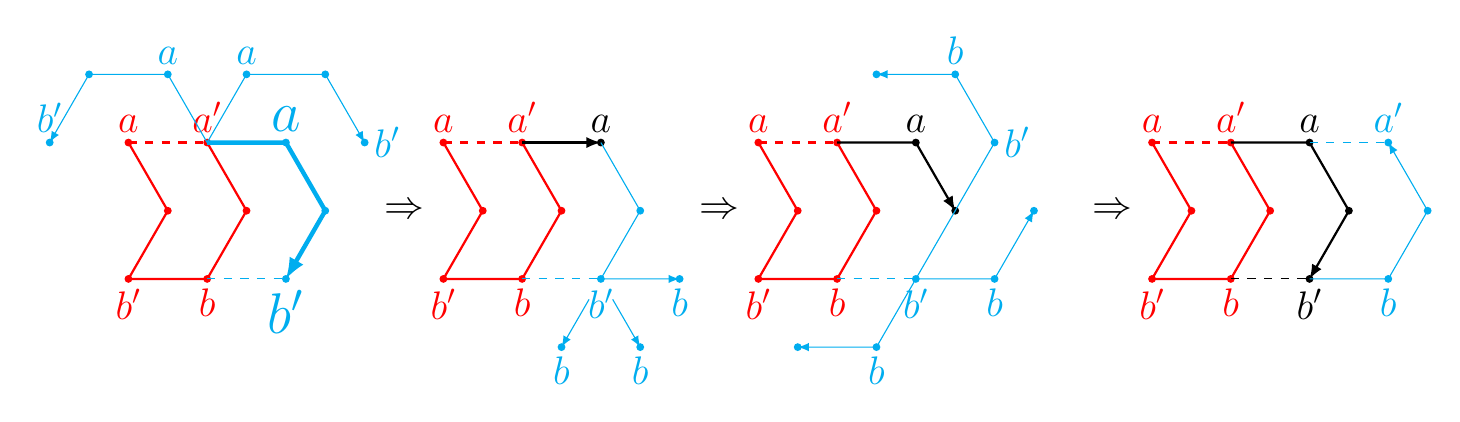
\begin{tikzpicture}
\tikzstyle{mol} = [fill,circle,inner sep=1pt]

\foreach \x in {0, 4, 8, 13} {
\draw[thick, red] (\x, 0) node[mol] {} node[above] {\Large $a$}
-- ++(300:1) node[mol] {} 
-- ++(240:1) node[mol] {} node[below] {\Large $b'$}
-- ++(0:1) node[mol] {} node[below] {\Large $b$}
-- ++(60:1) node[mol] {} 
-- ++(120:1) node[mol] {} node[above] {\Large $a'$}
;
\draw[thick, dashed,red] (\x, 0) -- ++(0:1);
}

\draw[cyan, -latex] (1, 0) -- ++(120:1) node[mol] {} node[above] {\Large $a$} -- ++(180:1) node[mol]{} -- ++(240:1) node[mol] {} node[above] {\Large $b'$};
\draw[cyan, -latex] (1, 0) -- ++(60:1) node[mol] {} node[above] {\Large $a$} -- ++(0:1) node[mol] {} -- ++(300:1) node[mol] {} node[right] {\Large $b'$};
\draw[ultra thick, cyan, -latex] (1, 0) -- ++(0:1) node[mol] {} node[above] {\huge $a$} -- ++(300:1) node[mol] {} -- ++(240:1) node[mol] {} node[below] {\huge $b'$};

\draw[dashed, cyan] (0,0)++(300:2) -- ++(0:1);

\draw (3,0)++(300:1) node {\Large $\Rightarrow$};
\draw (7,0)++(300:1) node {\Large $\Rightarrow$};
\draw (12,0)++(300:1) node {\Large $\Rightarrow$};


\draw[thick, -latex] (5, 0) -- ++(0:1) node[mol] {} node[above] {\Large $a$};

\draw[cyan, -latex] (6, 0) -- ++(300:1) node[mol] {} -- ++(240:1) node[mol] {} node[below] {\Large $b'$} -- ++(0:1) node[mol] {} node[below] {\Large $b$};
\draw[cyan, -latex] (5,0)++(300:2)++(240:0.3) -- ++(240:0.7) node[mol] {} node[below] {\Large $b$};
\draw[cyan, -latex] (5,0)++(300:2.3) -- ++(300:0.7) node[mol] {} node[below] {\Large $b$};
\draw[dashed, cyan] (4,0)++(300:2) -- ++(0:1);


\draw[thick, -latex] (9, 0) -- ++(0:1) node[mol] {} node[above] {\Large $a$}
-- ++(300:1) node[mol] {}
;
\draw[cyan, -latex] (10,0)++(300:1) -- ++(240:1) node[mol] {} node[below] {\Large $b'$}
-- ++(240:1) node[mol] {} node[below] {\Large $b$}
-- ++(180:1) node[mol] {}
;
\draw[cyan, -latex] (9,0)++(300:2) -- ++(0:1) node[mol] {} node[below] {\Large $b$} -- ++(60:1) node[mol] {};
\draw[cyan, -latex] (10,0)++(300:1) -- ++(60:1) node[mol] {} node[right] {\Large $b'$}
-- ++(120:1) node[mol] {} node[above] {\Large $b$}
-- ++(180:1) node[mol] {}
;
\draw[cyan,dashed] (8,0)++(300:2) -- ++(0:1);

\draw[thick, -latex] (14, 0) -- ++(0:1) node[mol] {} node[above] {\Large $a$}
-- ++(300:1) node[mol] {}
-- ++(240:1) node[mol] {} node[below] {\Large $b'$}
;
\draw[dashed] (13,0)++(300:2) -- ++(0:1);
\draw[cyan, -latex] (14,0)++(300:2) -- ++(0:1) node[mol] {} node[below] {\Large $b$}
-- ++(60:1) node[mol] {}
-- ++(120:1) node[mol] {} node[above] {\Large $a'$}
;
\draw[cyan,dashed] (15,0) -- ++(0:1);

\end{tikzpicture}}
\caption{Progression of a glider by distance 1.}
\label{fig:glider}
\vspace*{-3mm}
\end{wrapfigure}
%\end{figure}

%\begin{example}\label{ex:glider}
%A motif called the \emph{glider} explains well how oritatami systems behave. 

Let us provide an example of deterministic cyclic OS that folds into a motif of great use called the \textit{glider}. 
Let $\Sigma = \{a, a', b, b', \bullet\}$. 
Consider a delay-3 OS whose transcript $w$ is a repetition of $a \bullet b' b \bullet a'$ and whose rule set is $\mathcal{H} = \{(a, a'), (b, b')\}$, which makes $\bullet$-beads inert. 
By the fragment $w[1..3] = a \bullet b'$, the seed of this OS, colored in red in Fig.~\ref{fig:glider}, can be elongated in various ways, only three of which are shown in Fig.~\ref{fig:glider} (left). 
The only bead on the fragment capable of a new h-interaction is $b'$ (with a $b$-bead according to $\mathcal{H}$), and for that, the fragment must be folded as bolded in Fig.~\ref{fig:glider} (left). 
The first bead $w[1] = a$ is hence stabilized to the east of the previous bead, and then the bead $w[4] = b$ is transcribed. 
The next two beads $w[2], w[3]$ are stabilized as illustrated one after another, but we can easily see that the bolded elongation dominates even their stabilization. 
It suffices to observe that neither $w[4]$ nor $w[5]$ can form any new h-interaction. 
When $w[4] = b$ is transcribed (after $w[1]$ is stabilized), $b'$-beads around are either too far or too close  (recall that $w[4]$ cannot interact with $w[3] = b'$). 
In addition, $w[5]$ is inert. 
Thus, they cannot override the bolded ``decision.''
It is easily induced inductively that gliders of arbitrary ``flight distance'' can be folded. 

Gliders also provide a medium to propagate 1-bit at arbitrary distance as the position of their last beads, which is determined by the height (top or bottom) of the first bead and a flying distance.  
%The height (top or bottom) of the first bead determines whether the last bead is stabilized top or bottom after flying a given distance.
For instance, the glider in Fig.~\ref{fig:glider} launches top and thus its last bead (the $a'$) also comes top after traveling the distance 2.
The OS we shall propose exploits this information-carrying capability.
%\end{example}

Denote the points in $\mathbb{R}^2$ that correspond to vertices of $\mathbb{T}$ by $\mathbb{Z}_\bigtriangleup^2$. 
A \textit{shape} $S$ is a set of points on the triangular grid. 
For an integer $c \ge 1$, let $Rhomb_c = \{(x, y) \in \mathbb{Z}_{\bigtriangleup}^2 \mid x, y \le c\}$.
Let $S' = \{(cx, cy) \mid (x, y) \in S\}$. 
The \textit{$c$-rhombus scaling} of $S$ is the union over all $\vec{p} \in S'$ of sets of points $Rhomb_c + \vec{p} = \{\vec{v} \in R^2 \mid \mbox{$\vec{v} = \vec{r} + \vec{p}$ for some $\vec{r} \in Rhomb_c$}\}$.
%The \textit{$c$-rhombus scaling} of a shape $S$ is a shape obtained by expanding the distance between the points in $S$ equally by $c$ to obtain another shape $S'$ and replacing each point $\vec{p} \in S'$ by the rhombus whose sides are of length $c$. 
Let $\diamondsuit_c(S)$ be the $c$-rhombus scaling of $S$. 
We say that an OS $\Xi$ \textit{weakly folds} (or ``self-assembles'') $\diamondsuit_c(S)$ if every terminal assembly of $\Xi$ puts at least one bead in $Rhomb_c + \vec{p}$ for all $\vec{p} \in S$ and no bead in $Rhomb_c + \vec{q}$ for all $\vec{q} \not\in S$. 


%-------------------------------------------------------------------------------------------
	\section{Heighway dragon oritatami system}
%-------------------------------------------------------------------------------------------



We propose a generic design of deterministic oritatami system that allows us to fold an arbitrary finite portion of the Heighway dragon. 
%The design concept has been already explained in the introduction. 
The folded dragon is actually slanted as illustrated in Fig.~\ref{fig:heighway6_oritatami}, which is more natural than the conventional (upright) one to be folded over the triangular grid. 
Let $P[j_1 .. j_2]$ be the target portion and $n = \min\{m \mid j_2 < 2^m\}$. 
%Let $n$ be the minimum integer such that if the last turn of a target portion corresponds to $P[j]$, then $j \le n$. 
Independently of $n$, the design sets both delay and arity to 3 and employs 567 bead types and a fixed rule set $\mathcal{H}$ (some of the bead types could be saved but not easily due to the NP-hardness of minimizing the number of bead types \cite{HanKim2017}). 
The design challenges an extra requirement that the transcript be periodic; a periodic RNA transcript is likely to be transcribed out of a circular DNA sequence \cite{GearyAndersen2014}. 
Without requiring the periodicity, one could simply design left-turn and right-turn modules and concatenate their copies according to the paperfolding sequence $P$. 
Such a ``hardcoding'' goes against the spirit of algorithmic self-assembly, and an OS that folds into the infinite Heighway dragon, if any, could not take this approach in order to be describable by a finite mean. 


%Any finite portion of the Heighway dragon is expected to be foldable by \textit{hard-coding} if an arbitrary number of bead types is available and the shape can be scaled-up (though, if rescaling is not allowed, it is NP-hard to decide if for a given finite shape, there exists an oritatami system that folds into the shape \cite{PatitzRogers2017}). 
%The proposed design cannot take this approach because the number of bead types available is fixed. 
%An oritatami system $\Xi = (\mathcal{H}, \alpha, \delta, \sigma, w)$ that the design provides is periodic in the sense that its transcript is a periodic sequence. 
%If this system is for the $n$-th repetition of the Heighway dragon, then the length of its period is $|w|/2^{n-1}$. 
%One period corresponds to a successive two pairs of a red line segment and the following green L-shaped block. 

One period folds into successive two line segments of the dragon. 
Why do these segments have to be distinguished? 
The answer lies in that the dragon is slanted. 
The slanted dragon involves two types of left turn as well as two types of right turn: acute and obtuse. 
%Capability of one turning module to make all of the four possible turns would halve the period. 
%Such a turning module, however, would have to take quite a number of conformations; recall that what the module has to turn is not a straw but a thick wire through which the current count $i$ propagates. 
Capability of one turning module to make all of the four possible turns would halve the period but require quite a number of conformations. 
Recall that what the module has to turn is not a straw but a thick wire through which the count $i$ propagates. 
Such a module is too advanced for the current oritatami technology.  
Our approach makes it enough for a turning module to handle just two tasks: turning acutely and obtusely. 
Observe that after (slanted) vertical segments, the left turn is obtuse while the right turn is acute, whereas after horizontal ones, the left turn is acute while the right turn is obtuse. 
%In addition, we know \textit{a priori} which segments are vertical and which are horizontal; indeed vertical segments and horizontal segments occur alternately on the Heighway dragon. 
Moreover, vertical and horizontal segments occur alternately on the dragon. 
%Hence, we can attach a proper interpreter \textit{a priori} to each DFAO module to convert its output L/R into a signal A(cute)/O(btuse). 
The alternation enables to endow each segment with a proper interpreter \textit{a priori} of the direction L/R, computed through a line segment, into a signal A(cute)/O(btuse).  
Two types of interpreters are hence needed: the vertical one interprets L as O and R as A, while the horizontal one does conversely. 

\begin{figure}[tb]
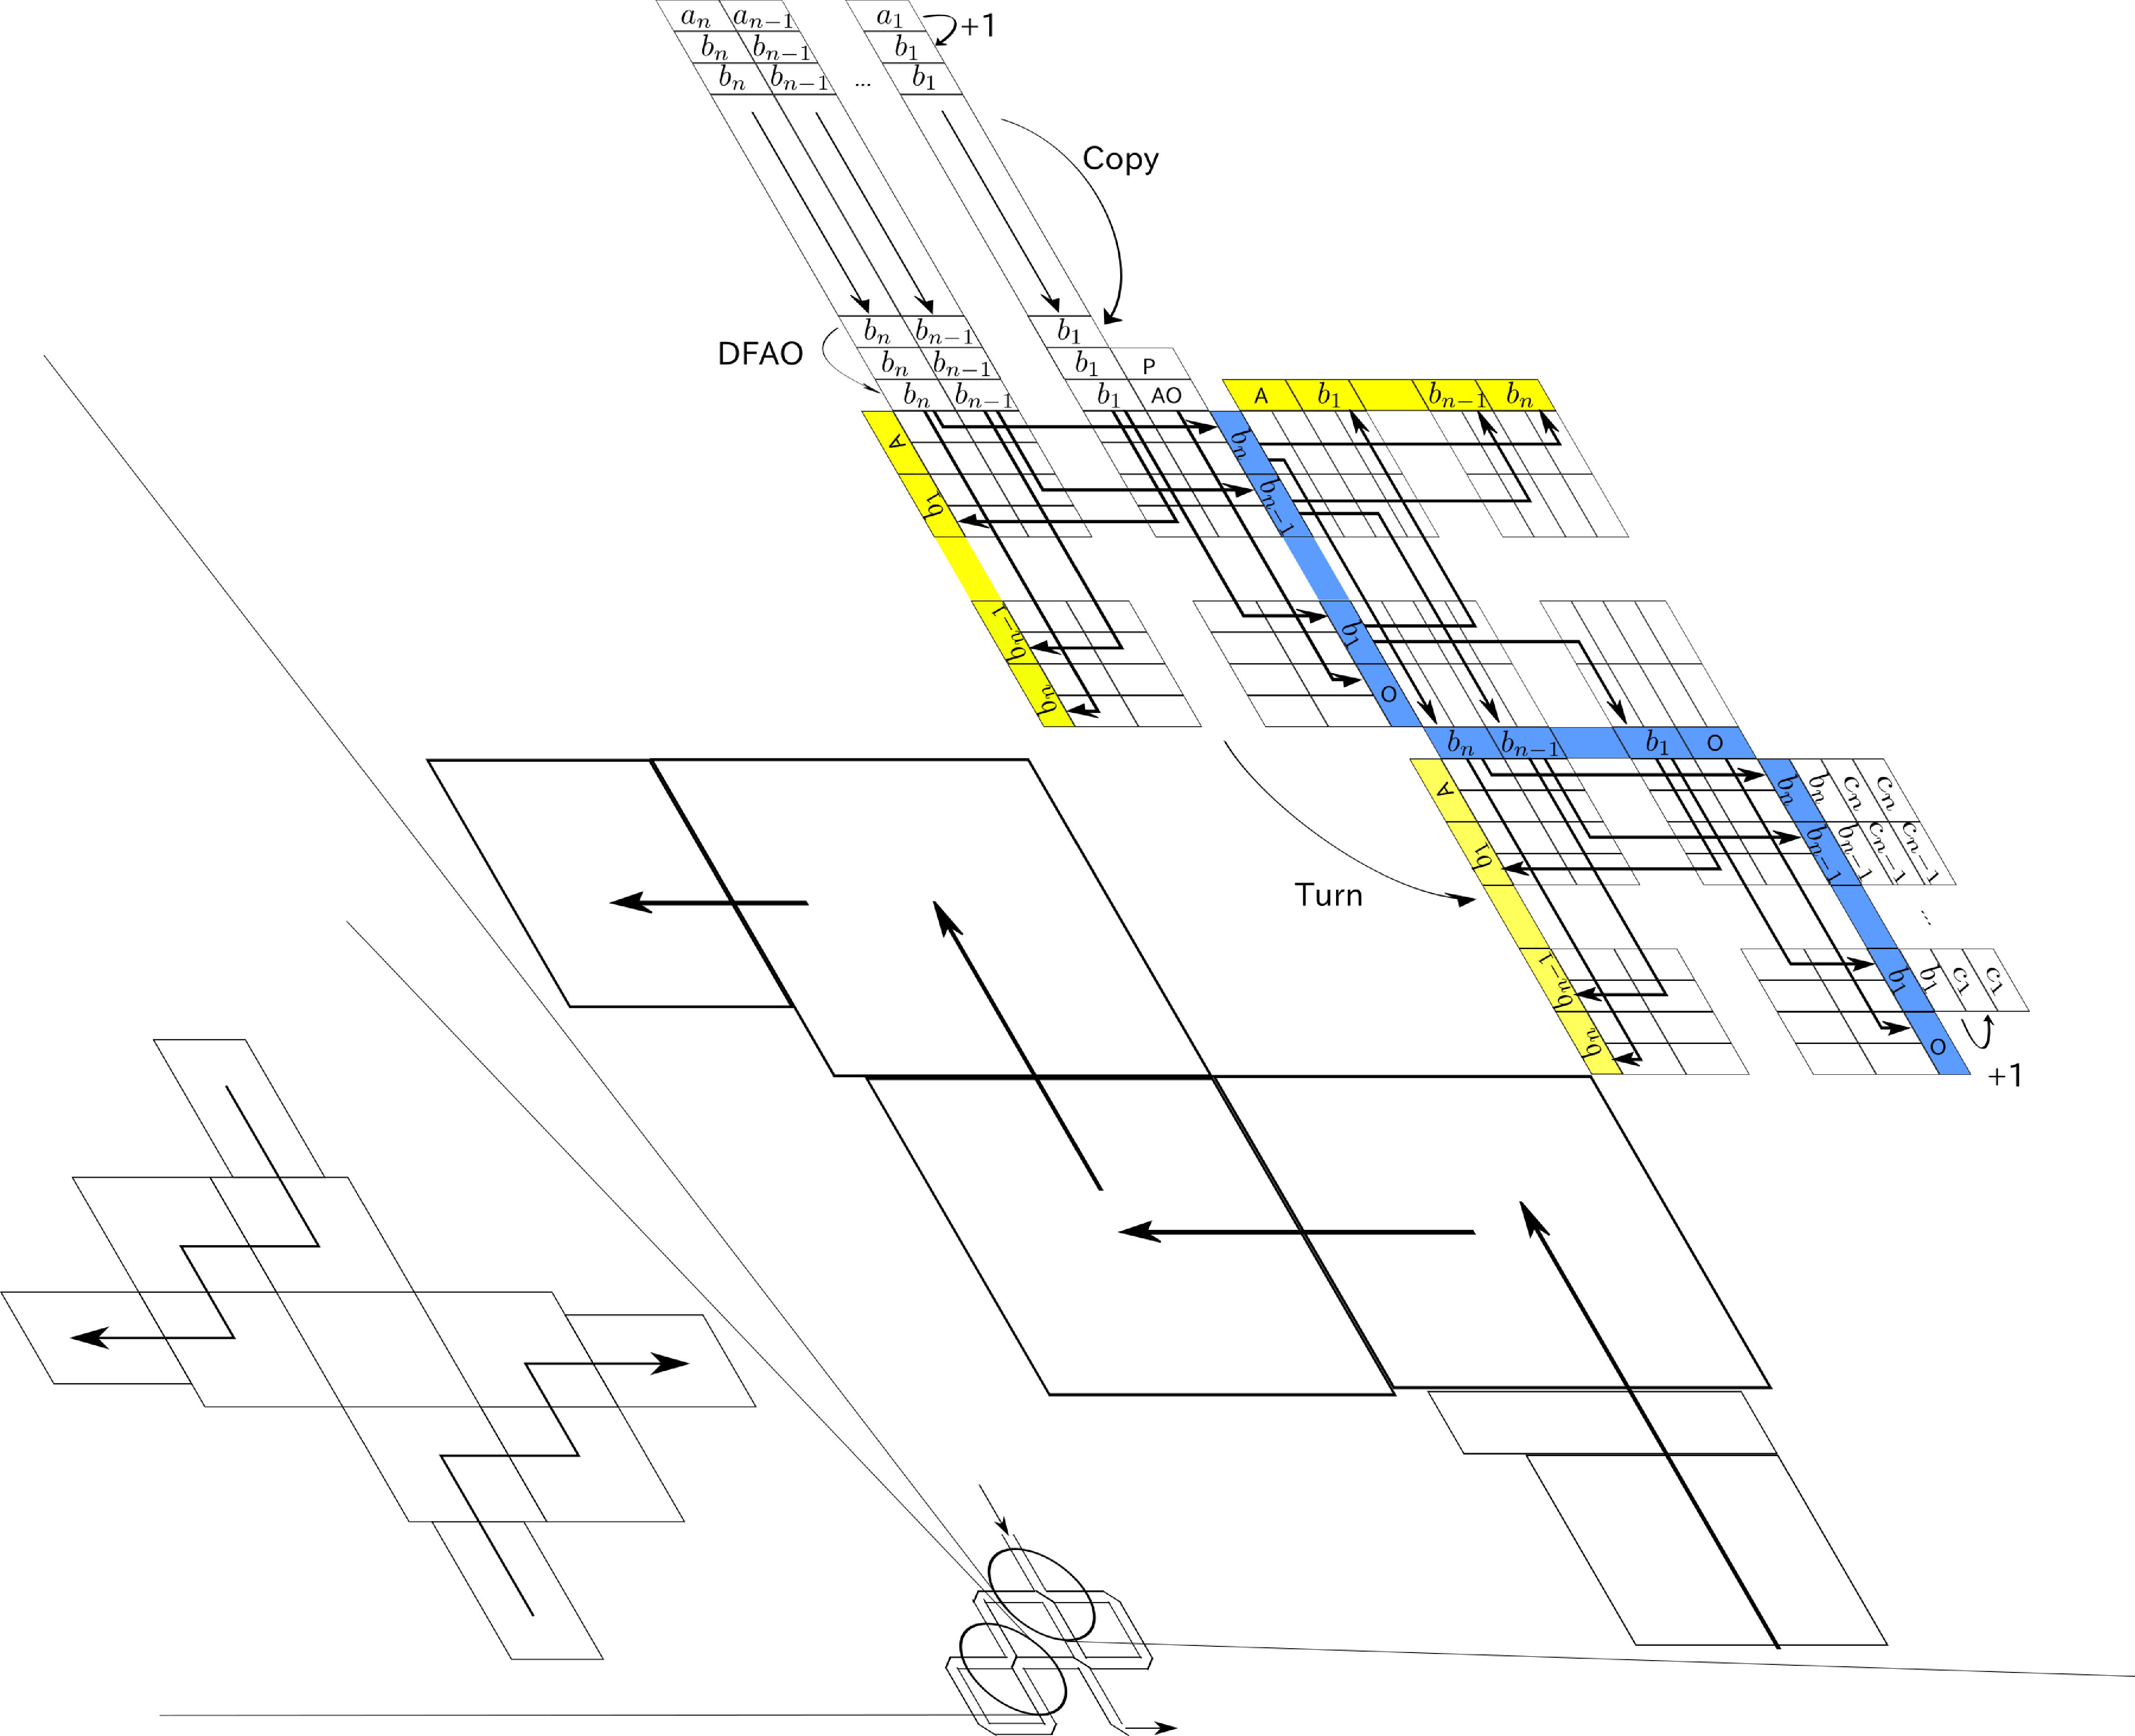
\includegraphics[width=\linewidth]{pic/dragon_vol4.pdf}
\caption{
Folding of one segment plus turn of the Heighway dragon, flow of information through it, and the two ways of collision avoidance between two turns.
}
\label{fig:abst_dragon}
\end{figure}

The first and second halves of a period differ only in the type of interpreter (AO or $\overline{\rm AO}$) so that we just explain the first. 
%Its transcript consists of three subsequences respectively for the counters, DFAO, and turning modules. 
%It folds as abstracted in Fig.~\ref{fig:abst_dragon} into one line segment plus one turn of the dragon and has its three subsequences accomplish the following tasks, respectively: 
Its transcript folds as abstracted in Fig.~\ref{fig:abst_dragon} into one line segment plus one turn of the dragon. 
The transcript consists of three subsequences responsible for the following tasks, respectively:  
\begin{enumerate}[itemsep=0pt]
\item $i \gets i + 1$ and propagate $i$, drawing a line segment;
\item (DFAO module) Compute $P[i]$ and interpret it as either A or O;
\item (Turning module) Make a turn accordingly.
\end{enumerate}
The length of the half is proportional to $n^2$ and hence so is that of a period. 
The seed of the system replaces the first counter module of the first period and encodes the initial count $j_1$ as a sequence of bead types in a format that the following counters can ``read.'' 
We shall explain how modules read something later. 
Before explaining the implementation of each module, we should point out one significant issue specific to the folding by oritatami systems. 
It rises when the dragon makes a turn where it has already turned before, that is, when two turns share a point. 
By definition, oritatami systems cannot put a bead anywhere occupied by another bead. 
This is the reason of the L-shape of the turning module. 
As shown in Figs.~\ref{fig:heighway6_oritatami} and \ref{fig:abst_dragon}, the proposed system makes an acute turn by having three bifurcation components direct the growth of further folding acutely one after another, while it makes an obtuse turn by having them direct the growth rather obtusely. 

%-------------------------------------------------------------------------------------------
%		\subsection{Modules}
%-------------------------------------------------------------------------------------------

Now it suffices to explain how modules and their components have been implemented, interlocked with each other, and collaborate. 
Using the simulator developed for \cite{HaKiOtSe2016}, we verified that all of the components fold correctly in all possible environments, which are abstracted in Figs.~\ref{fig:abst_dragon}, \ref{fig:abst_dfao}, and \ref{fig:overall_turning}. 

%-------------------------------------------------------------------------------------------
			\subsubsection{Counter module}
%-------------------------------------------------------------------------------------------

The existing binary counter \cite{GeMeScSe2016} was modified so as to operate in the dynamics \eqref{eq:cotranscriptional_folding}, which is more prevailing \cite{HanKim2017,HaKiOtSe2016,OtaSeki2017} though less tractable. 

%%%%%%%%%%%%%%%%%%%%%%%%%%%%%%%%%%%%%%%%%%%%
%\begin{figure}[h]
\begin{wrapfigure}{r}{0.6\linewidth}
\vspace*{-5mm}
\centering
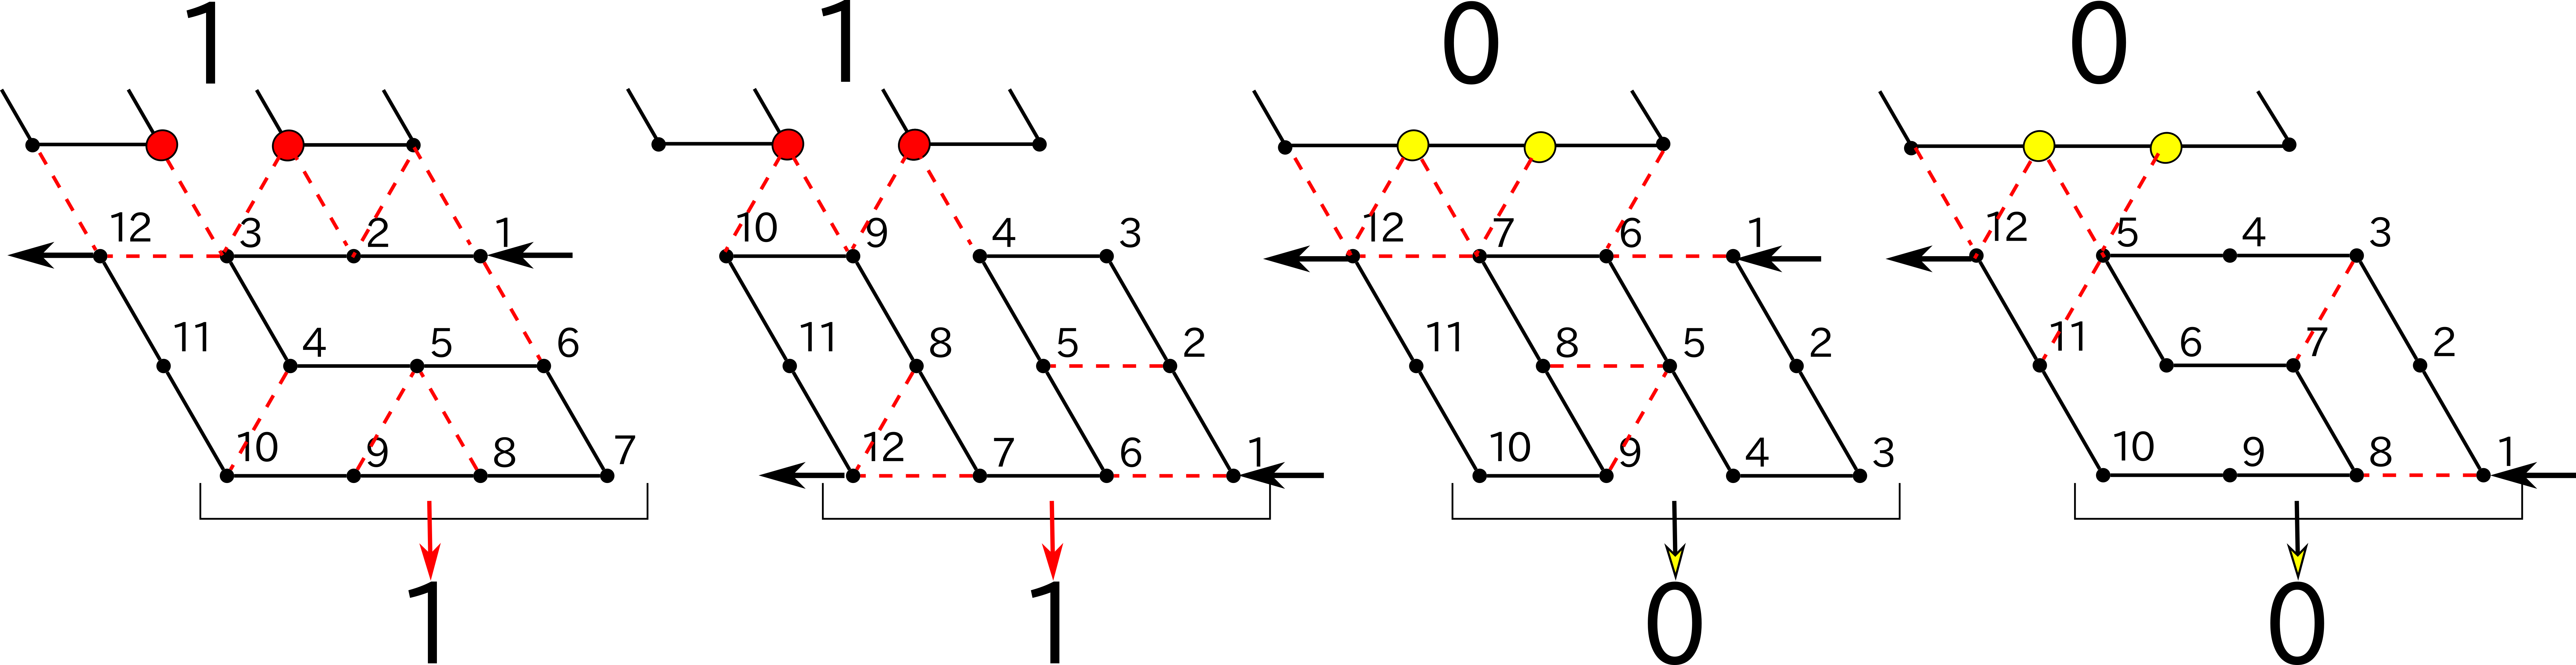
\includegraphics[width=\linewidth]{pic/counter_zig.png}
\caption{All conformations of the half-adder.
The first and third are diverted to implement the body-lpx2 component of the turning module. 
}
\label{fig:half-adder}
\vspace*{-3mm}
\end{wrapfigure}
%\end{figure}
%%%%%%%%%%%%%%%%%%%%%%%%%%%%%%%%%%%%%%%%%%%%

A counter module for $n$-bit sequences is a catenation of the following components in the order: right-turner, $n$ half-adders, left-turner, and $n$ formatters. 
It folds into one zigzag. 
Suppose each bit of an $n$-bit input $a_n a_{n-1} \cdots a_1$ is given as a specific sequence of 4-bead types as suggested in Fig.~\ref{fig:half-adder} and the input is provided as the catenation of such bit sequences for $a_n, a_{n-1}, \ldots, a_1$. 
The right-turner folds in such a way that the first bead of the first half-adder comes at a distance of either 1 or 3 southeastward from the rightmost bead of the LSB $a_1$. 
Thus, the first half-adder encounters only the four surrounding environments (contexts) shown in Fig.~\ref{fig:half-adder}, in which the half-adder, or actually its transcript {\tt 1}-{\tt 2}-\dots-{\tt 12}, folds deterministically as illustrated, or more precisely, the generic rule set $\mathcal{H}$ is designed so as for the transcript to favor the illustrated conformation the most in each context. 
Interpret the first bead {\tt 1} (resp.~last bead {\tt 12}) being far from the input as carry-in (resp.~carry-out) and close as no carry-in (resp.~no carry-out). 
Then we can see carry be out only when $a_1 = 1$ and carry is in (the second context in Fig.~\ref{fig:half-adder}). 
Being concatenated, half-adders ripple carry from one to the other. 
The half-adder can expose four sequences below: {\tt HA-1a}, {\tt -0a}, {\tt -0b}, and {\tt -1b}. 
They are pairwise distinct enough for another component to ``read'' the output. 
After the left-turner guides the counter module from its zig to zag, $n$ formatters format each bit as {\tt HA-1a/1b} $\to$ {\tt HA-1} and {\tt HA-0a/0b} $\to$ {\tt HA-0} using its two conformations. 
Thus, a counter module increments an input by 1 if its first half-adder is fed with carry (i.e., the right-turner locates its {\tt 1} away from $a_1$), or just propagates it otherwise. 
Concatenating counter modules and feeding carry-in only to the first one yields a line segment through which the current count $i$ is incremented by 1 and propagated through. 

\begin{comment}
A counter module folds into one zigzag. 
Its essential component is the half-adder. 
The first half of its transcript is a catenation of $n$ half-adders. 
In Fig.~\ref{fig:abst_dragon}, half-adders are abstracted as small parallelograms at the top labeled with $a_n$, $a_{n-1}$, $\ldots$, $a_1$, where the one with $a_j$ is for the $j$-th bit of the current count $i$. 
%Though not described, two horizontally adjacent half-adders sandwitch a glider of even length as a space to keep them away from each other sufficiently to prevent any undesirable interference. 
As illustrated in Fig.~\ref{fig:half-adder}, the whole system is designed in such a manner that a half-adder starts folding at one of two positions (top/bottom) relative to the 1-bit input (0/1) that is encoded as a sequence of bead types colored in red or yellow and it folds into one of the four possible conformations. 
Starting at the bottom should be interpreted as carry-in while at the top as no carry-in, and the position of ending should be interpreted analogously for carry-out. 
%The whole system is designed in such a manner that a 1-bit input (1 or 0) is exposed to the specific position (colored red or yellow in Fig.~\ref{fig:half-adder}) as a pair of bead types by the previous turning module. 
%The system is also designed in such a manner that a half-adder starts folding either at the top, as in the first and third conformations, or at the bottom as in the other two. 
%The half-adder considers starting at the top as non-carry and at the bottom as carry. 
%Thus, only when a half-adder takes 1 and carry, it ends at the bottom (second conformation in Figure~\ref{fig:half-adder}), which is propagated to the next half-adder as it is via the spacer between them. 
These four conformations expose sequences of four bead types below that are distinct enough to convey the intended 1-bit output to another computing component, or in other words, we can design a component that can ``read'' the output. 
From this point forward, conformations for other components will be illustrated; their input and output will be labeled by their meaning mutually understood by the components that exchange them. 
Observe that a half-adder can output 1 in two different formats {\tt HA-1a} and {\tt HA-1b} and also 0 as {\tt HA-0a} and {\tt HA-0b}. 
The role of the zag is to reformat them into {\tt HA-1} and {\tt HA-0} so that other components can read them easily. 
A counter module either increments an input by 1 if being fed with carry, or propagates the input otherwise. 
%Being fed with non-carry, the counter module serves as the copier module. 
\end{comment}

%-------------------------------------------------------------------------------------------
			\subsubsection{DFAO module}
%-------------------------------------------------------------------------------------------


As abstracted in Fig.~\ref{fig:abst_dfao}, a DFAO module receives the current count $i$ from the previous counter module, computes $P[i]$, interprets it properly either A or O, and outputs it together with the count $i$. 

\begin{figure}[h]
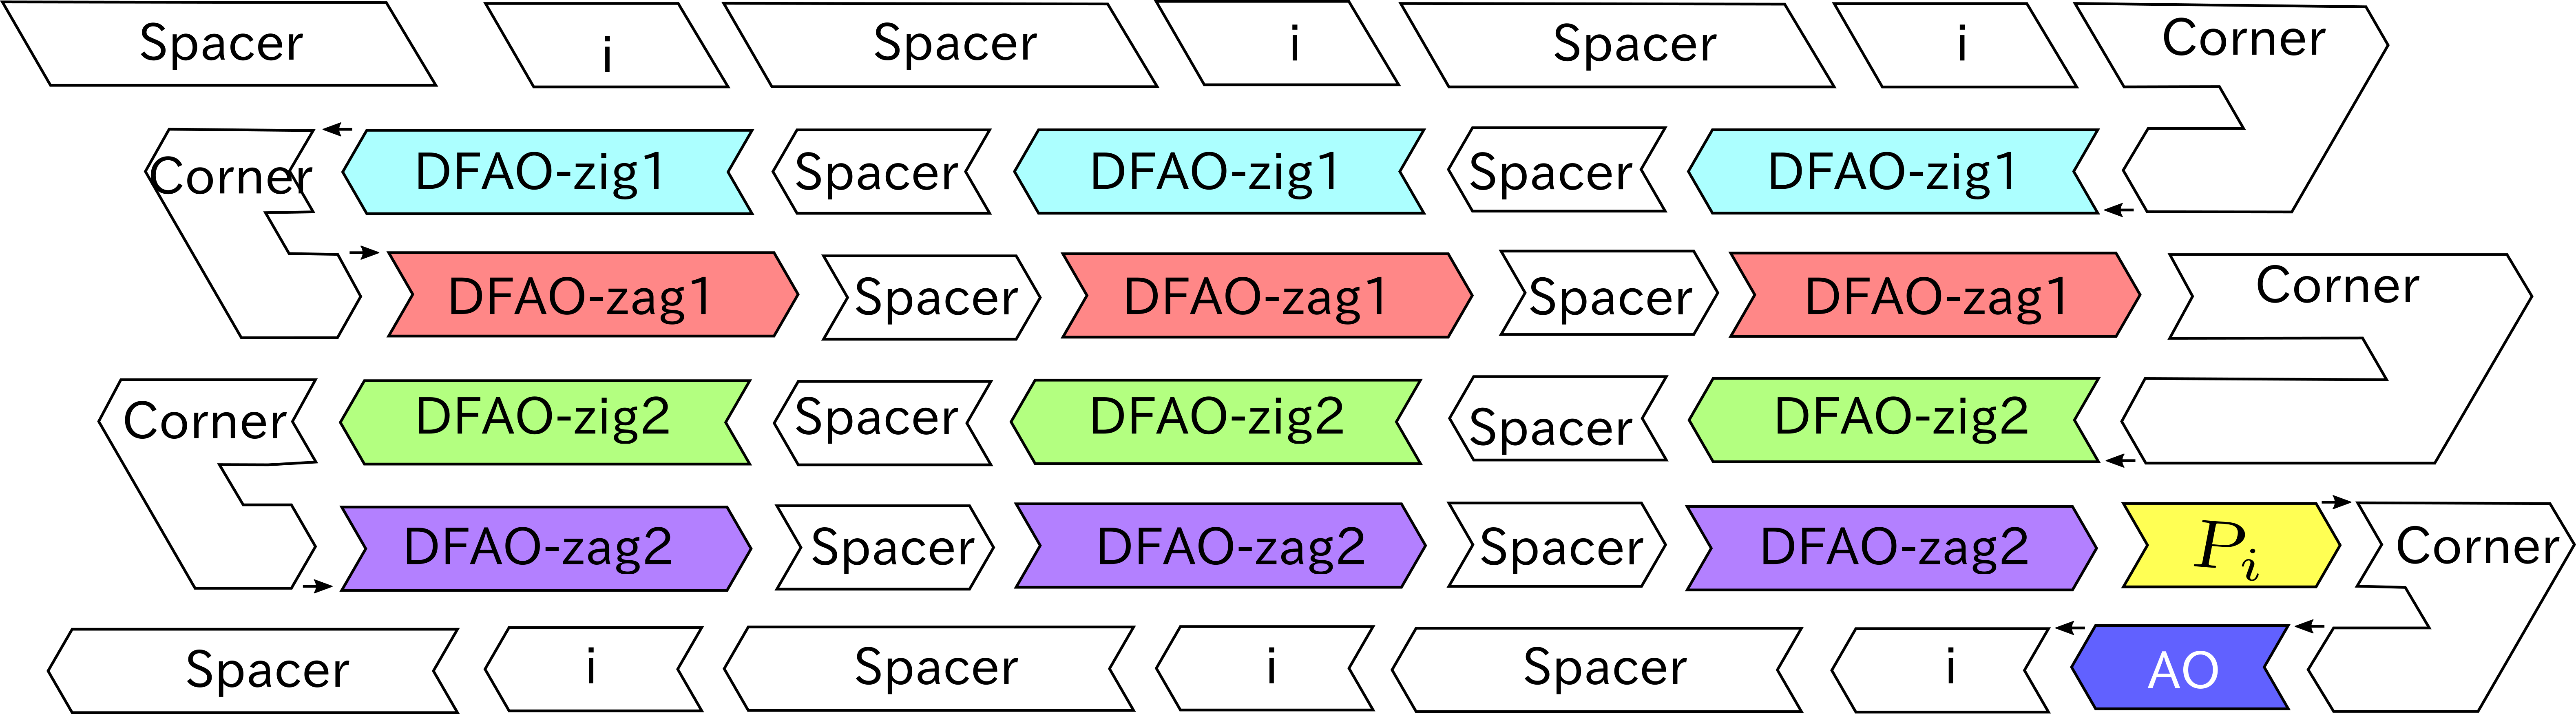
\includegraphics[width=\linewidth]{pic/abst_DFAO.png}
\caption{Component-level abstraction of the folding of DFAO module.}
\label{fig:abst_dfao}
\end{figure}

%%%%%%%%%%%%%%%%%%%%%%%%%%%%%%%%%%%%%%%%%%%%

\begin{figure}[h]
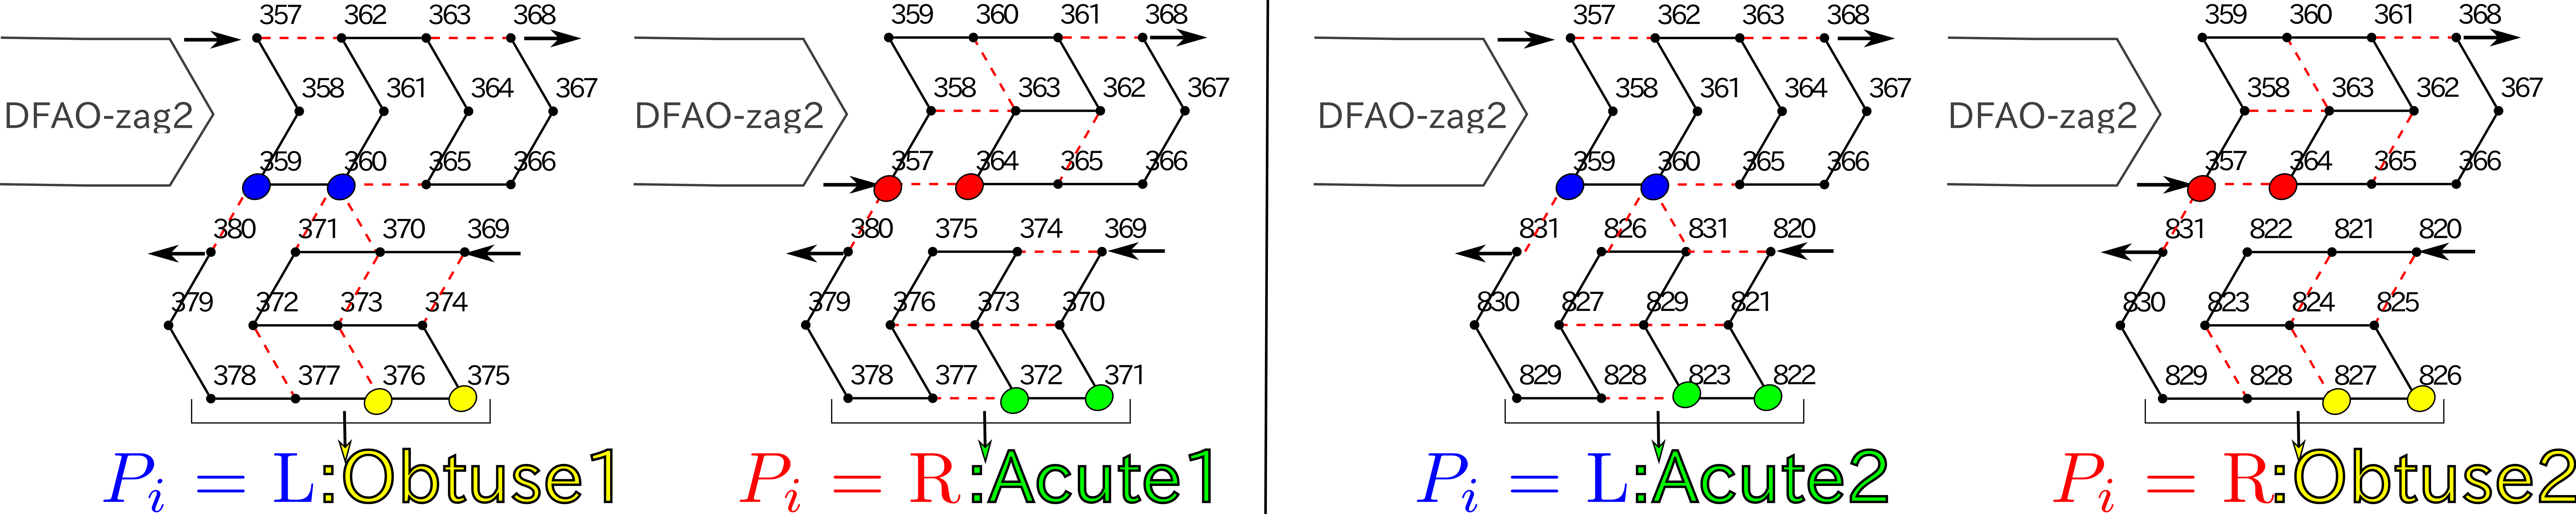
\includegraphics[width=\linewidth]{pic/PFS.png}
\caption{The two conformations of PFS above and the corresponding two conformations of (left) AO and (right) of $\overline{\rm AO}$.}
\label{fig:PFS}
\end{figure}
%%%%%%%%%%%%%%%%%%%%%%%%%%%%%%%%%%%%%%%%%%%%


The DFAO module is composed of the six components: DFAO-zig1, DFAO-zag1, DFAO-zig2, DFAO-zag2, PFS, and AO (or  ``$\overline{\rm AO}$").
It folds into two zigzags and one more zig.
In the first zigzag, DFAO-zig1's and -zag1's read $i$ from its LSB and ``mark" the first 0. 
In the second zigzag, DFAO-zig2's and -zag2's check whether the marked 0 is followed by 0 ($P[i] = L$) or 1 ($P[i] = R$) and have PFS output $P[i]$ downward (see Fig.~\ref{fig:PFS} also for AO and $\overline{\rm AO}$). 
The last zig is equipped with AO if this module is for a vertical segment or with $\overline{\rm AO}$ otherwise; AO interprets the output L of PFS as obtuse and A as acute, while $\overline{\rm AO}$ interprets them the other way around. 
%The second zag is to end at the top if $P[i] = L$ or at the bottom if $P[i] = R$.
%PFS takes one of the two conformations in Fig.~\ref{fig:PFS} and outputs $P[i]$ downward.
%In vertical segments, AO interprets the output L as obtuse and R as acute as shown in Fig.~\ref{fig:PFS} (left), while in horizontal ones $\overline{\rm AO}$ interprets them the other way around as shown in Fig.~\ref{fig:PFS} (right). 
Let us explain briefly how each of the components folds to fulfill its roles.

%%%%%%%%%%%%%%%%%%%%%%%%%%%%%%%%%%%%%%%%%%%%
%\begin{figure}[h]
\begin{wrapfigure}{r}{0.65\linewidth}
\vspace*{-5mm}
\centering
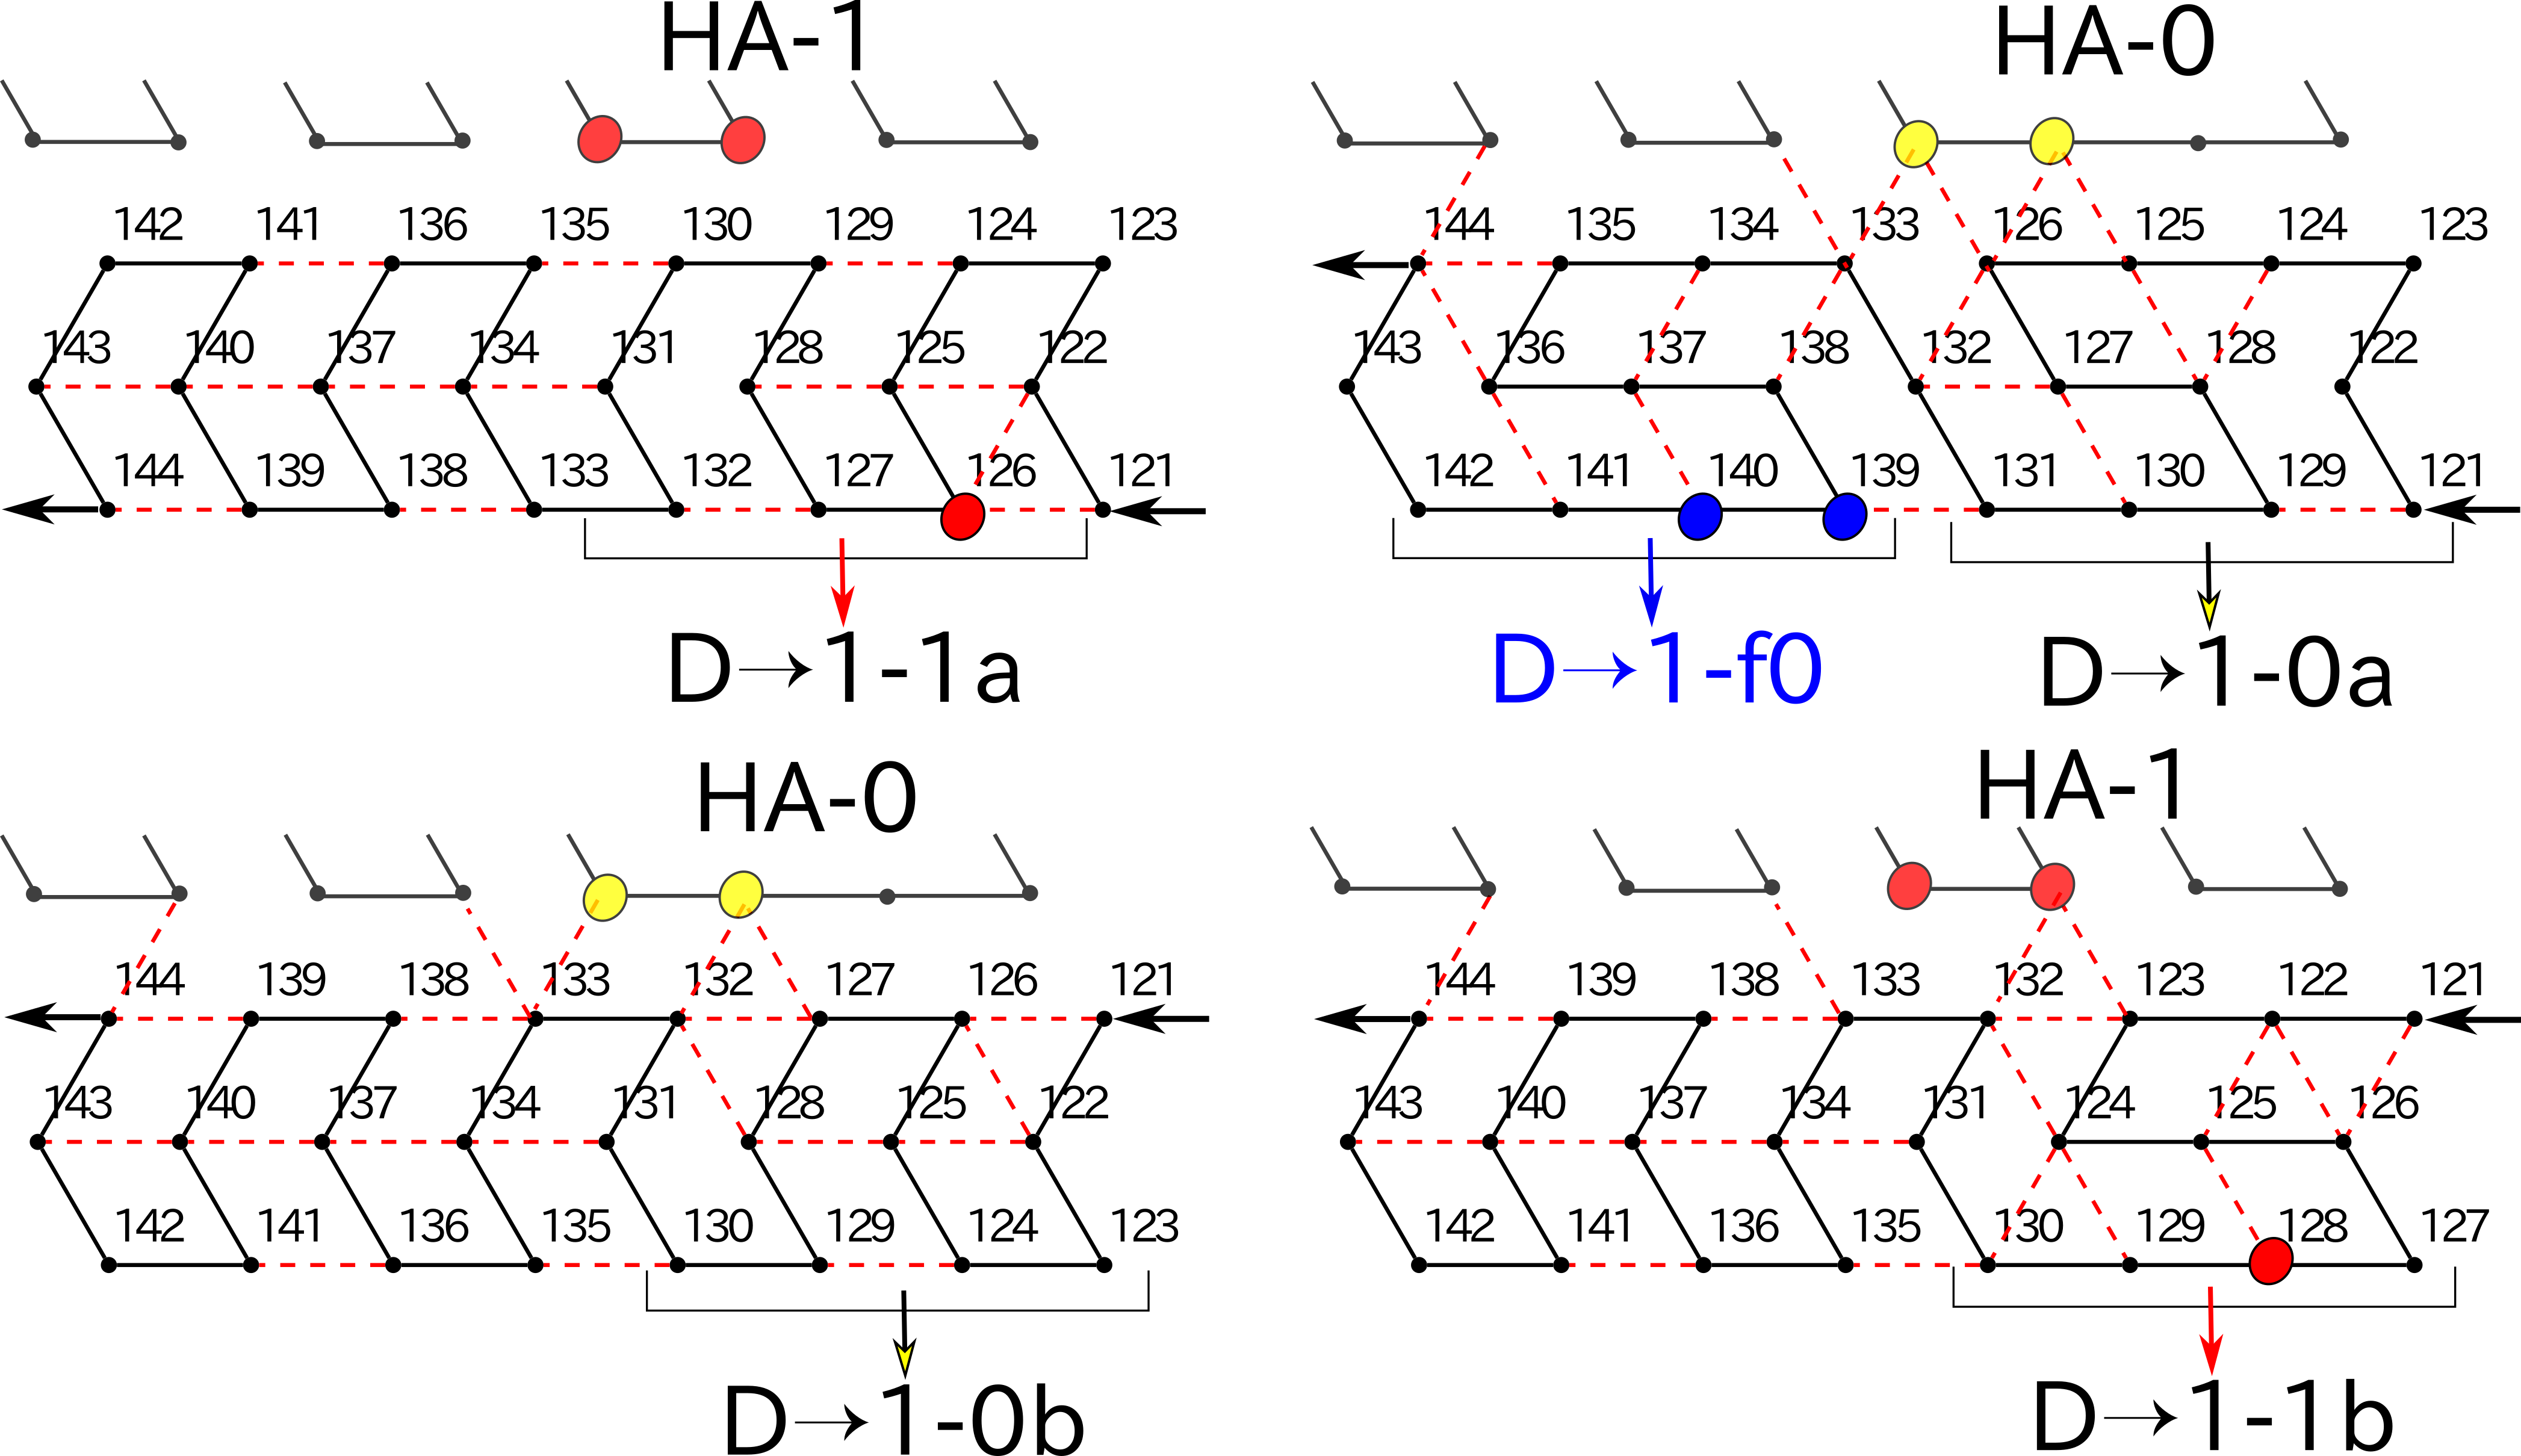
\includegraphics[width=\linewidth]{pic/DFAO-zig1.png}  
\caption{The four conformations of DFAO-zig1: (top) Dzig1-1 and Dzig1-f0; (bottom) Dzig1-20 and Dzig1-21.}
\label{fig:DFAO-zig1}
\vspace*{-3mm}
\end{wrapfigure}
%\end{figure} 

DFAO-zig1's collaboratively detect the first 0 read from the LSB in two phases.
See Fig.~\ref{fig:DFAO-zig1} for its possible contexts and corresponding conformations. 
Phase1 is to copy all the 1's prior to the first 0 and Phase2 is to copy all the bits after the first 0.
These phases are distinguished by the relative position where a DFAO-zig1 starts folding to the input (far in Phase~1 while close in Phase~2).
In Phase1, DFAO-zig1s certainly take the conformation Dzig1-1 (the top left one in Fig.~\ref{fig:DFAO-zig1}).
At the first 0, a DFAO-zig1 folds into Dzig1-f0 instead, ending at the top in order to transition to Phase~2.
Each of the succeeding DFAO-zig1s takes Dzig1-20 or -21 to copy all the remaining bits. 
Note that there is a cushion between two DFAO-zig1s called \textit{spacer}.
Spacers are used to prevent undesirable interference among components.
They are implemented as a glider (see Sect.~\ref{sect:preliminaries}), hence capable of propagating 1bit on which phase the system is in.
In the first zag, DFAO-zag1's just propagate 0's, 1's, and the first 0 using the three conformations in Fig.~\ref{fig:DFAO-zag1}.



%%%%%%%%%%%%%%%%%%%%%%%%%%%%%%%%%%%%%%%%%%%%
\begin{figure}[h]
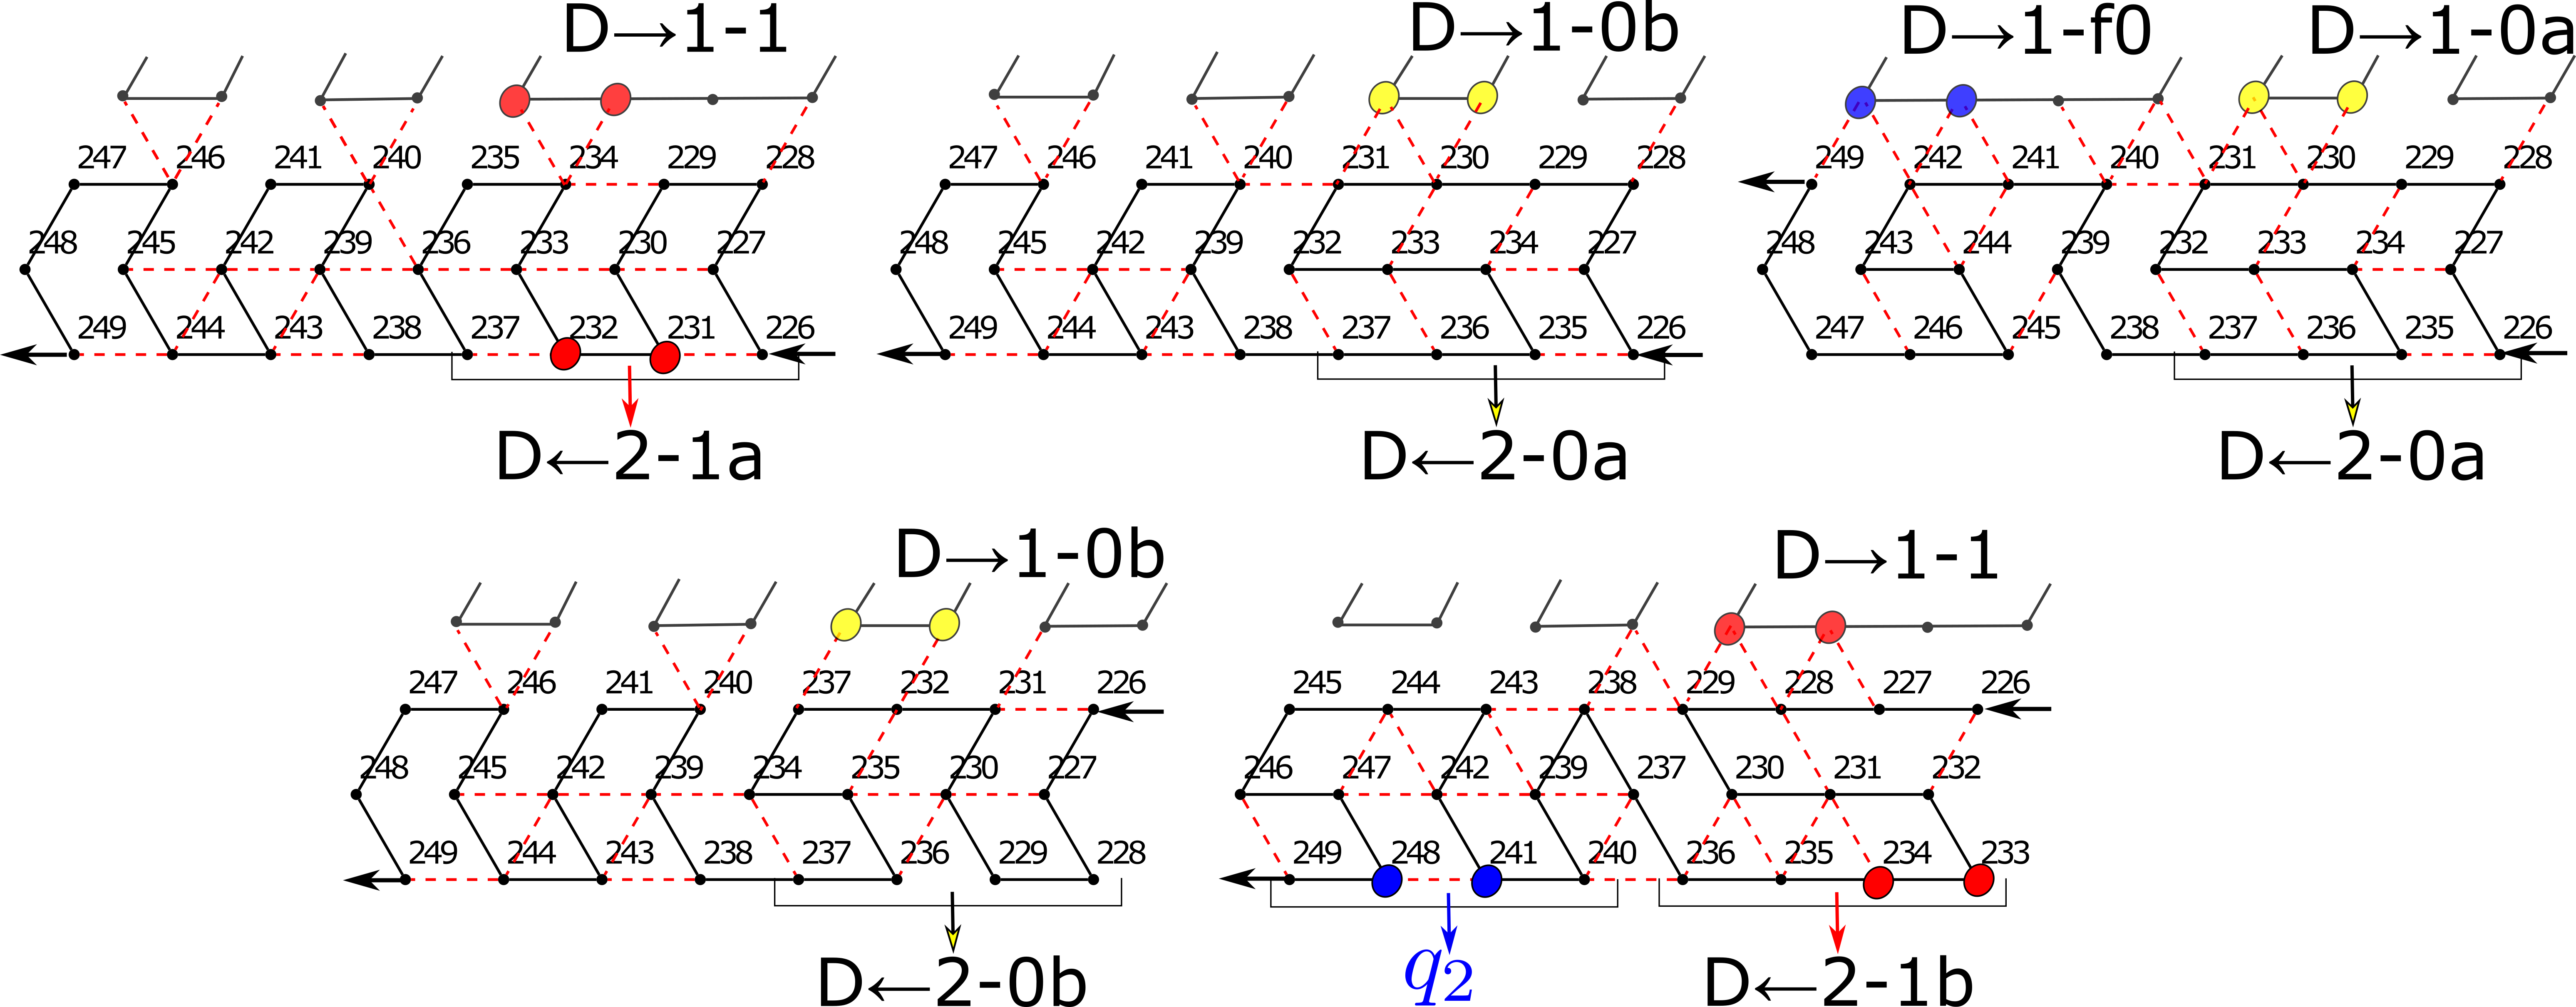
\includegraphics[width=\linewidth]{pic/DFAO-zig2.png}
  \caption{The five conformations of DFAO-zig2: (top) Dzig2-1, Dzig2-0, Dzig2-f0, (bottom) Dzig2-f00, and Dzig2-f01. }
  \label{fig:DFAO-zig2}
\end{figure} 

%%%%%%%%%%%%%%%%%%%%%%%%%%%%%%%%%%%%%%%%%%%%%%%%
\begin{figure}[h]
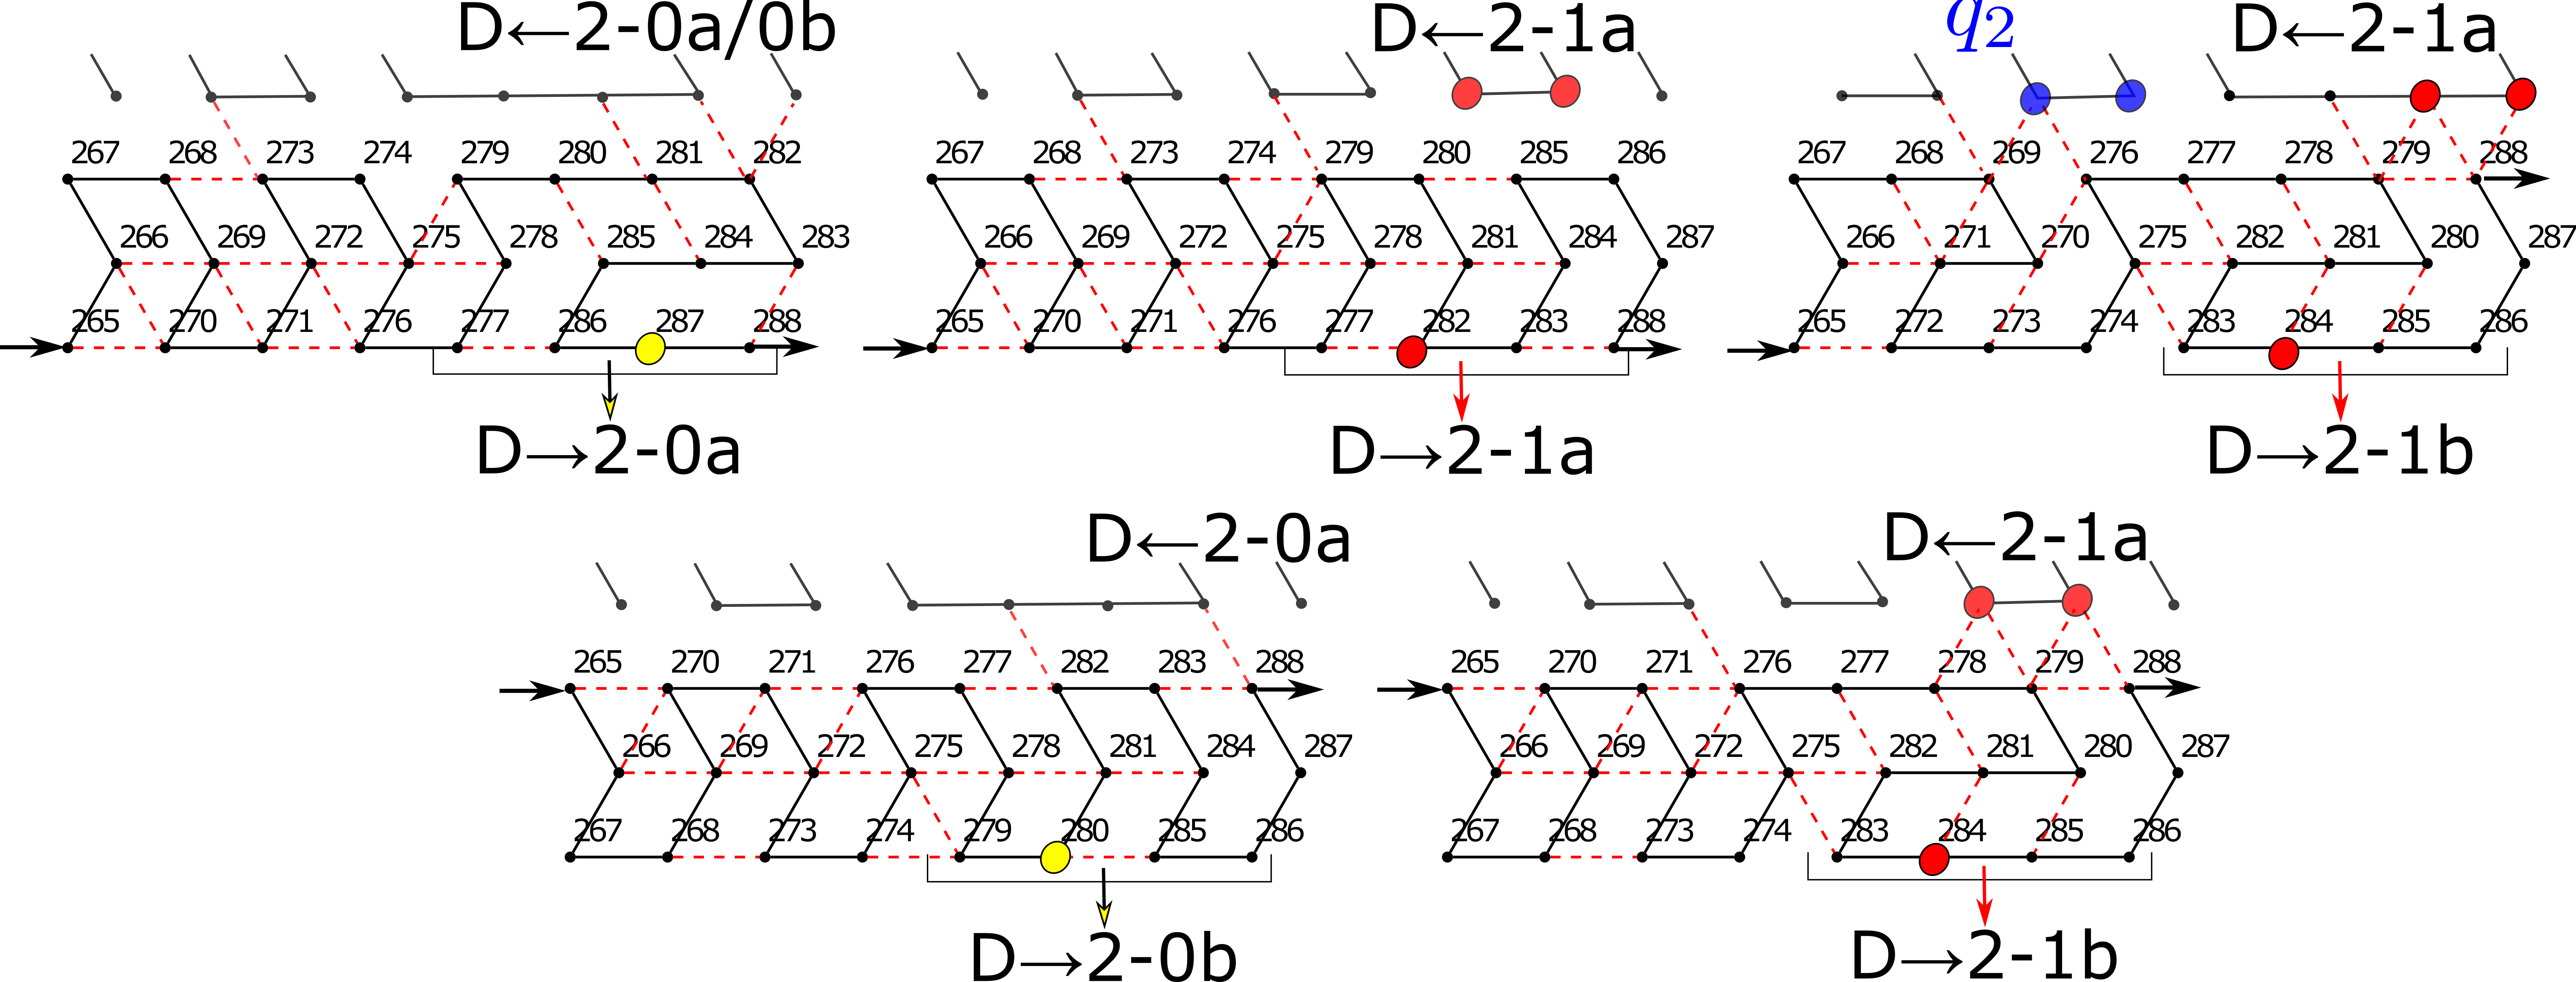
\includegraphics[width=\linewidth]{pic/DFAO-zag2.png}
\caption{The five conformations of DFAO-zag2: (top) Dzag2-L0, Dzag2-L1, Dzag2-T1, (bottom) Dzag2-R0, and Dzag2-R1.
The first and second halves are diverted to implement the body-rgy and body-gx components of the turning module, respectively. 
}
\label{fig:DFAO-zag2}
  \end{figure} 
%%%%%%%%%%%%%%%%%%%%%%%%%%%

In the second zig, DFAO-zig2's check whether the first 0 is followed by 0 or 1, being read from LSB.
They first copy the 1's by the conformation Dzig2-1 (top left in Fig.~\ref{fig:DFAO-zig2}) until the first 0, read from the LSB, which is distinguished from the other 0's by the mark. 
Starting at the bottom and reading 0, the DFAO-zig2 can take two conformations Dzig2-0 and -f0.
They share the first half.
The marker f0 folds the second half so as to end at the top, yielding Dzig2-f0. 
The next DFAO-zig2 therefore starts to fold at the top so that it takes one of the two conformations Dzig2-f00 and -f01 depending on the bit read.
Recall that reading 1 here is equivalent to transitioning to $q_2$, that is, $P[i] = L$.
Observe that Dzig2-f01 is provided with the marker $q_2$, which lets the DFAO-zag2 component below know $P[i] = L$. 
These conformations end at the bottom.
The remaining 0's and 1's are copied by Dzig2-0 and -1.
The second zag starts at the bottom and copy 0's and 1's by the two conformations Dzag2-L0 and -L1 of DFAO-zag2 (top left and center in Fig.~\ref{fig:DFAO-zag2}) until a DFAO-zag2 encounters the 1 marked by $q_2$, if any. 
At the encounter, the DFAO-zag2 takes the special conformation Dzag2-T1 and changes the ending position to the top, letting the remaining DFAO-zag2s rather take Dzag2-R0 and -R1 for copying, which end at the top.
As such, the second zag can feed $P[i]$ to PFS as the position of its first bead.

%The third zig lets $P[i]$ go through its AO (or $\overline{\rm AO}$) component to be reinterpreted either as A(cute) or as O(btuse) and propagates the current count $i$.   


%%%%%%%%%%%%%%%%%%%%%%%%%%%%%%%
%-------------------------------------------------------------------------------------------
			\subsubsection{Turning module}
%-------------------------------------------------------------------------------------------

\begin{figure}[t]
\centering
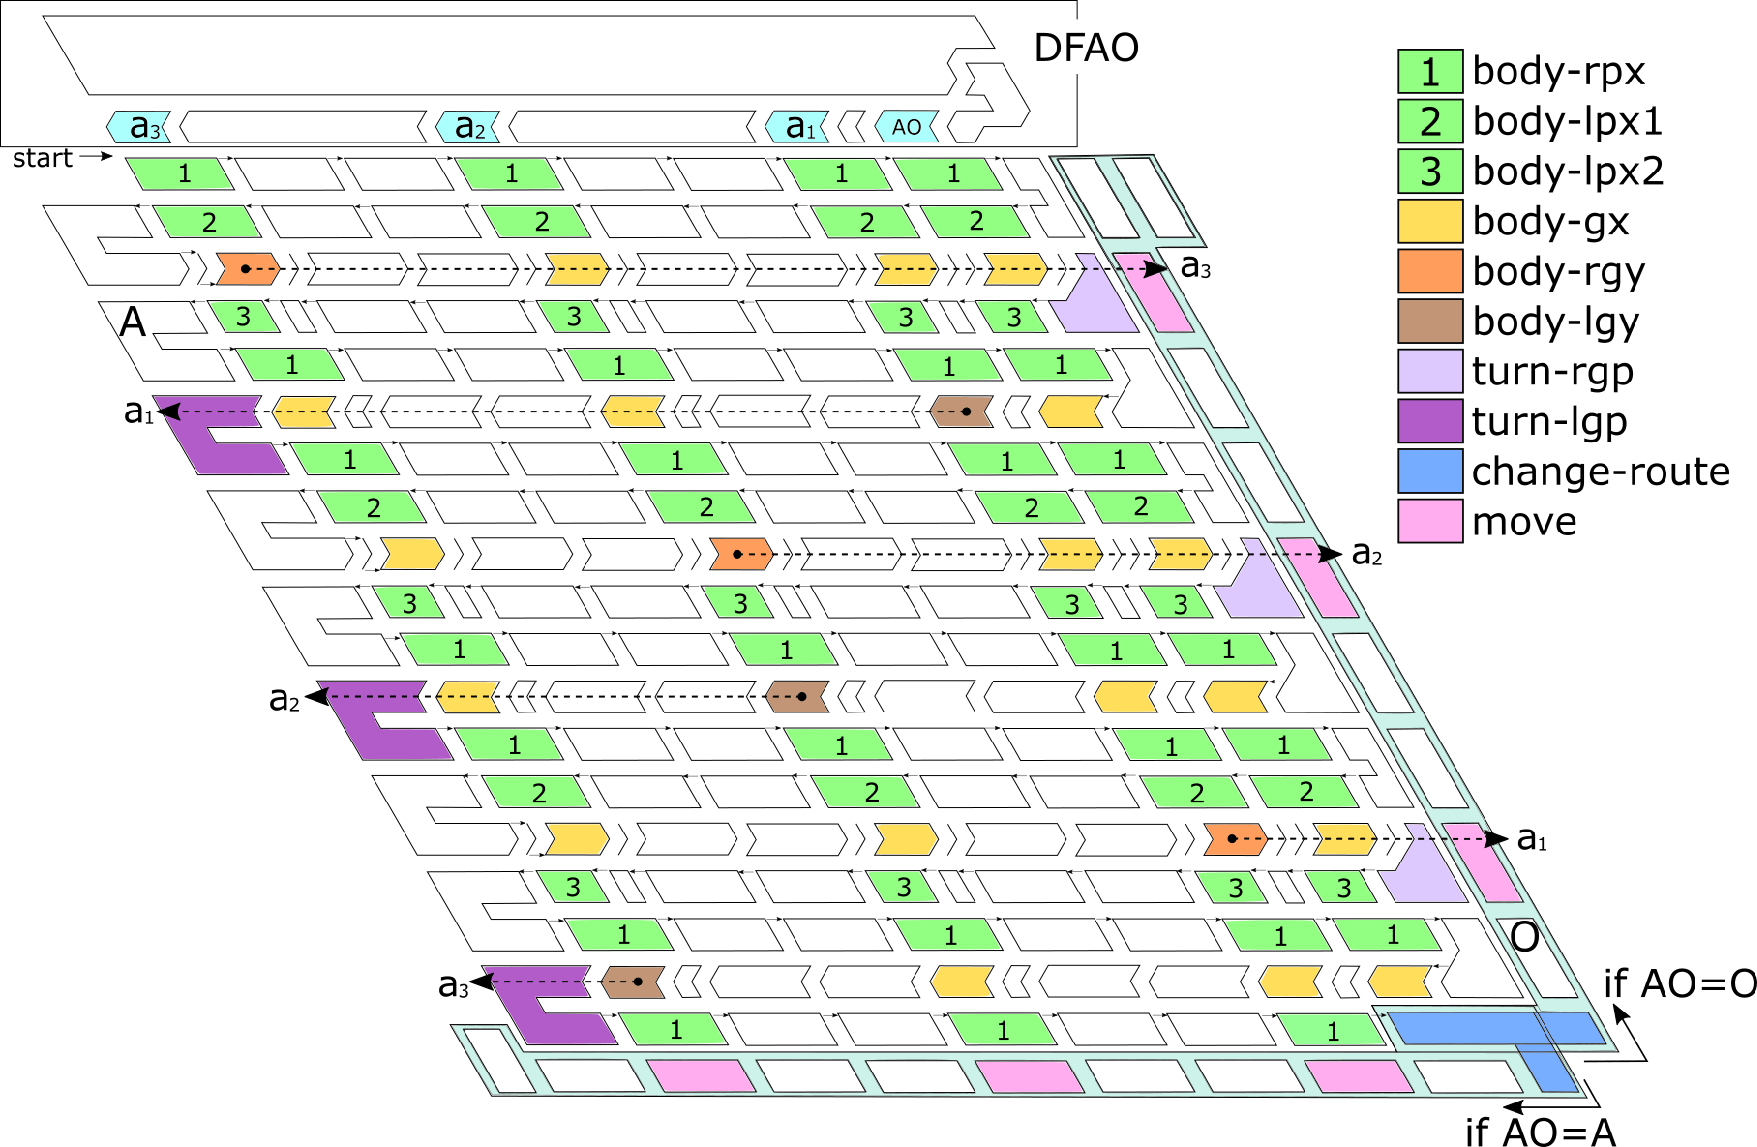
\includegraphics[width=\linewidth]{pic/overall_turn_part.pdf}
\caption{
Component-level abstraction of folding of turning module.
All the white components in the middle are spacers, some of which are implemented in the shape of parallelogram instead of glider. 
 }
\label{fig:overall_turning}
\end{figure}

The last module is for turn. 
It consists of two submodules: bit-sequence bifurcator and steering arm (shaded in light blue in Fig.~\ref{fig:overall_turning}). 

The bifurcator bifurcates the bits of the current count $i$ and the reinterpreted signal (A or O) as shown in Fig.~\ref{fig:abst_dragon} while folding into zigzags.
For that, it employs components to handle the following four types of tasks: 
\begin{enumerate}[itemsep=0pt]
\item propagate 1-bit vertically: body-rpx (Fig.~\ref{fig:body-rpx} (left)), body-lpx1 (Fig.~\ref{fig:body-rpx} (right)), and body-lpx2 (Fig.~\ref{fig:half-adder});
\item let 1-bit cross another 1-bit: body-gx (Fig.~\ref{fig:DFAO-zag2}); 
\item fork 1-bit vertically and horizontally: body-rgy (Fig.~\ref{fig:DFAO-zag2}) and body-lgy (Fig.~\ref{fig:body-lgy});  
\item undergo transition between a zig and a zag and exposes 1-bit outside: turn-rgp (Fig.~\ref{fig:turn-rgp}) and turn-lgp (Fig.~\ref{fig:turn-lgp}). 
\end{enumerate} 
%that propagates 1bit vertically (body-rpx, body-lpx1, and body-lpx2 in Figure~\ref{fig:overall_turning}), that lets 1bit cross another 1bit (body-gx), that forks 1bit vertically and horizontally (body-rgy, body-lgy), and that undergoes transition from a zig to a zag or from a zag to a zig and exposes 1bit outside (turn-rgp, turn-lgp).
Components to handle the first two types of tasks have already been implemented (see, e.g., \cite{HaKiOtSe2016}) so that we shall explain the others.

%The component body-rgy takes one of the two conformations in Figure~\ref{fig:body-rgy} depending on the 1-bit encoded in the two beads above.
%Output below, the 1-bit is encoded as a type of the second bead from left, while output right, it is encoded as the position of its last bead (top or bottom).
%Its zag-variant, body-lgy, is implemented analogously; for its conformations.

%\begin{figure}[h]
\begin{wrapfigure}{r}{0.55\linewidth}
\vspace*{-5mm}
\centering
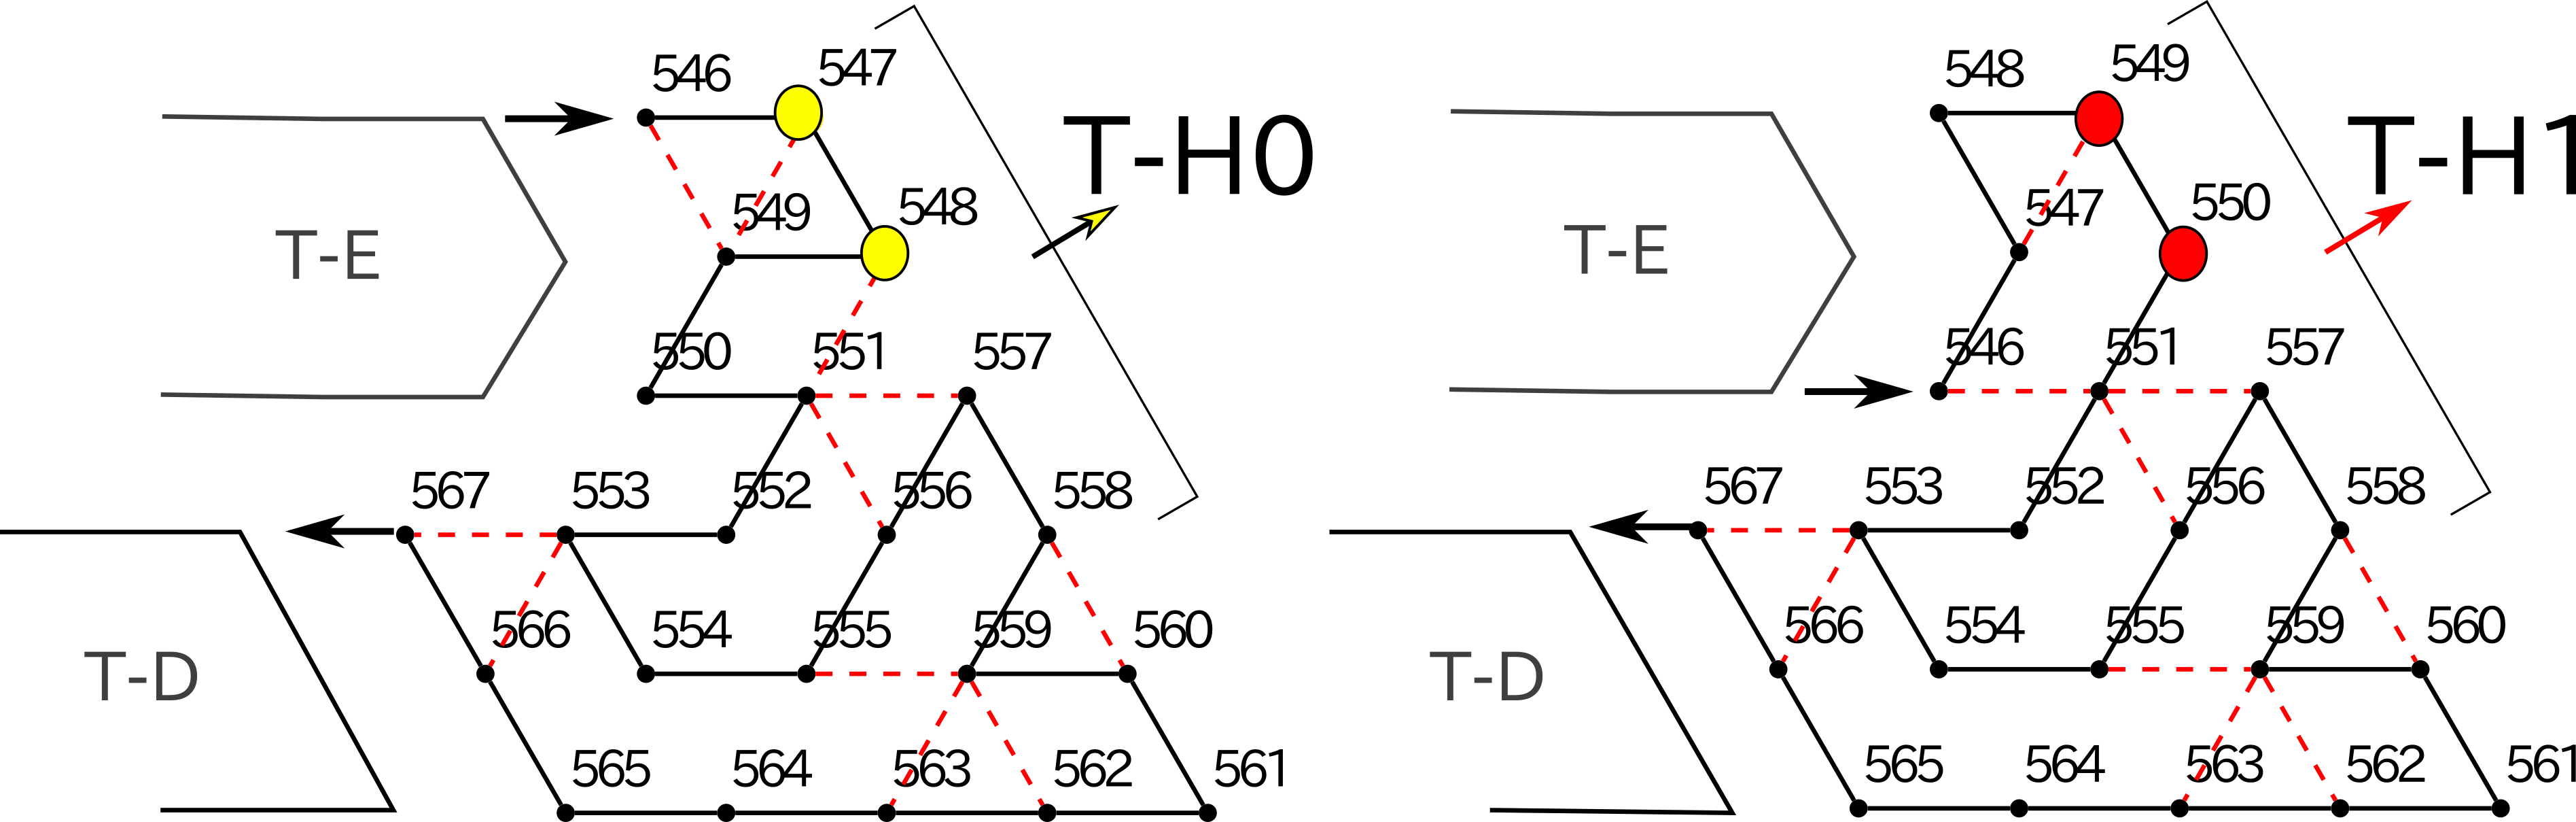
\includegraphics[width=\linewidth]{pic/turn-rgp.png}
\caption{The two conformations of turn-rgp.}
\label{fig:turn-rgp}
\vspace*{-3mm}
\end{wrapfigure}
%\end{figure}

The component body-rgy is implemented by reusing the first half of DFAO-zag2 (Fig.~\ref{fig:DFAO-zag2}). 
Starting from the bottom, it can take two conformations which end at different heights and expose sequences of bead types sufficiently pairwise distinct downward. 
Hence, we can divert it to fork 1bit input rightward and downward. 
The 1bit thus forked transfers till the end of a zag and is converted by the turn-rgp into a sequence of bead types (see Fig.~\ref{fig:turn-rgp}). 
The body-lgy and turn-lgp are their zig counterparts (Figs.~\ref{fig:body-lgy} and \ref{fig:turn-lgp}). 

%The 1bit forked rightward by a body-rgy transfers till the end of the zig without being jammed because all remaining modules in the zig are designed in such a way that they start and end at the same height like the even-distance glider.
%The module turn-rgp receives the 1bit (top or bottom), and exposes it by taking one of the two comformations in Figure~\ref{fig:turn-rgp}.
%The module turn-lgp functions analogously in zags as being folded in Figure~\ref{fig:turn-lgp}.

\begin{figure}[h]
\centering
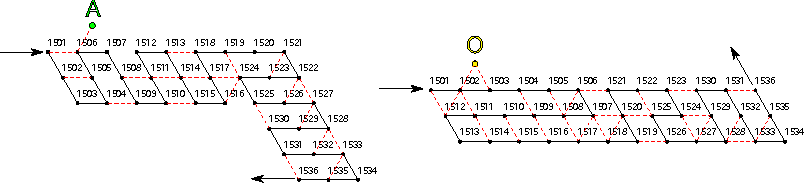
\includegraphics[width=\linewidth]{pic/change_route.pdf}
\caption{The two conformations of change-route.}
\label{fig:change_route}
\end{figure}

The bifurcator also propagates the 1-bit A/O, output by the DFAO module, to tell the steering arm which way it should take.
Specifically, the signal has the component, change-route, of the steering arm take one of the two conformations in Fig.~\ref{fig:change_route}, guiding the rest of the arm towards the specified direction.
The remaining arm is a catenation of move components (Fig.~\ref{fig:move}), which is capable of letting the bifurcated bit sequence through.  
Note that the turning module need not bifurcate AO.
Indeed, the second and third turning modules are supposed to turn in the same manner as the first one.
It hence suffices to append A and O to the bifurcated bit sequences on the acute side and obtuse side, respectively, as shown in Fig.~\ref{fig:overall_turning}.

\begin{remark}
As suggested in Fig.~\ref{fig:overall_turning}, the bifurcation component actually outputs an input bit sequence also downward.
That is, it trifurcates the input.
This provides a more space-efficient way to replicate a bit sequence many-folds.
\end{remark}


%%%%%%%%%%%%%%%%%%%%%%%%%%%%%%%


%--------------------------------------------------------
	\section*{Acknowledgements}
%--------------------------------------------------------

We would like to thank Hwee Kim and Aleck Johnsen for their helpful advices and discussions.





%-------------------------------------------------------------------------------------------
	\bibliographystyle{plain}
	\bibliography{oritatami}
%-------------------------------------------------------------------------------------------

\end{document}
